% Section 6: Numerical Examples

\textbf{Design.} We compute summary statistics for the \emph{myopic mean-field consistent dynamics} in Sections~II--IV using a particle approximation: simulate $N$ agents with shared common shocks $(W,U,Z)$ and independent idiosyncratic signal noises $\{B_i\}$, with trading governed by the myopic rule \eqref{eq:myopic_policy} and belief updates given by the Kalman filter in Appendix~A (implemented in discrete time via Euler/Kalman recursions). We report four baseline scenarios:
(i) bull regime ($\mu_v>0$) with $k=1$,
(ii) bull regime with $k=3$,
(iii) bear regime ($\mu_v<0$) with $k=1$,
(iv) bear regime with $k=3$.
Each scenario is averaged over $M$ independent random seeds.

\textbf{Implementation.} \ifjeicblind Simulations and plotting are reproducible from the replication package. Link omitted for blind review. \else Simulations and plotting are reproducible from the repository using
\texttt{code/scripts/}\allowbreak\texttt{build\_paper\_artifacts.py}, which writes run-level CSVs and aggregated figures into \texttt{paper\_artifacts/}. \fi Table~\ref{tab:params} lists the baseline parameters.
The baseline parameters satisfy the per-step contraction/uniqueness condition $0\le B_t<\Delta t$ (Theorem~\ref{thm:contraction}), uniformly along the simulated path.
Unless otherwise stated, we use time step $\Delta t=1$; Table~\ref{tab:dt_sensitivity} reports a coarse time-step sensitivity check.
\textbf{Timing.} Within each discrete step $t\to t+1$ (decision interval $\Delta t$), agents:
(i) observe their private signal increment (equivalently, the normalized increment $z_{i,t}=(\xi_{i,t+\Delta t}-\xi_{i,t})/\Delta t$) and update $(\hat v_{i,t},\Sigma_{i,t})$;
(ii) compute the post-trade mean inventory $\bar x_t$ from the closed-form stock--flow fixed point using the pre-trade mean $\bar x_{t^-}=\bar x_{t-1}$ (Proposition~\ref{prop:step_fixed_point});
(iii) set $\bar u_t=(\bar x_t-\bar x_{t-1})/\Delta t$;
(iv) compute each agent's post-trade inventory $x^\star_{i,t}$ from the myopic rule given $\bar u_t$ and set $u_{i,t}=(x^\star_{i,t}-x_{i,t^-})/\Delta t$ with $x_{i,t^-}=x_{i,t-1}$;
(v) update price via flow impact, $\Delta p_{t+1}=\kappa(v_t-p_t)\Delta t+\lambda\bar u_t\Delta t+\phi\sqrt{\Delta t}\,\varepsilon_{t+1}$;
(vi) update wealth $W_{i,t+1}=W_{i,t}+x^\star_{i,t}\Delta p_{t+1}-(\chi/2)(x^\star_{i,t})^2\Delta t$; and
(vii) set next pre-trade inventory $x_{i,t+1^-}=x^\star_{i,t}$.
In the price-augmented robustness variant, agents then incorporate $p_{t+1}$ via the implicit observation in Appendix~A (updating beliefs for time $t+1$). Thus, no future price information is used at decision time.

\begin{table}[t]
  \centering
  \scriptsize
  \setlength{\tabcolsep}{2pt}
  \renewcommand{\arraystretch}{1.15}
  \resizebox{\columnwidth}{!}{\begin{tabular}{p{0.18\linewidth} p{0.27\linewidth} p{0.30\linewidth} p{0.25\linewidth}}
\toprule
\textbf{Channel / mechanism} & \textbf{Analytic model (math)} & \textbf{Particle implementation (code)} & \textbf{Alignment / notes} \\
\midrule
\textbf{Time convention} &
Continuous time ($dt$); myopic rule uses infinitesimal scaling. &
Discrete grid with step $\Delta t$ (baseline $\Delta t=1$). &
State $\Delta t$ explicitly when translating between $dp_t$ and $\Delta p_{t+1}$. \\
\addlinespace
\textbf{Price formation} &
Anchored impact SDE $dp_t=\kappa(v_t-p_t)\,dt+\lambda\bar x_t\,dt+\phi\,dZ_t$. &
Euler update $p_{t+1}=p_t+\kappa(v_t-p_t)\Delta t+\lambda\bar x_t\Delta t+\phi\sqrt{\Delta t}\,\varepsilon^\eta_{t+1}$. &
Aligned up to discretization; $\phi$ is the reduced-form price-noise scale (microstructure sketch: $\phi=\lambda\sigma_\eta$). \\
\addlinespace
\textbf{Signal / observation} &
Flow signal $d\xi_{i,t}=v_t\,dt+\sigma_c\,dU_t+\sigma_\epsilon\,dB_{i,t}$. &
Normalized increment $z_{i,t}=(\xi_{i,t+\Delta t}-\xi_{i,t})/\Delta t$; for $\Delta t=1$, $z_{i,t}=v_t+\text{noise}$. &
Aligned; normalization makes the observation noise scale with $1/\sqrt{\Delta t}$. \\
\addlinespace
\textbf{Belief state} $(\hat v_{i,t},\Sigma_{i,t})$ &
Kalman--Bucy filter; $\Sigma$ solves Riccati. &
Discrete-time Kalman recursion for $(\hat v_{i,t},\Sigma_{i,t})$ (Appendix~A). &
Aligned at the state level. \\
\addlinespace
\textbf{Trading rule (risk term)} &
Continuous-time myopic CARA uses variance rate $\phi^2$ (drift uncertainty is $O(dt^2)$). &
One-step mean--variance uses $\Var_{i,t}(\Delta p_{t+1})=\phi^2\Delta t+\kappa^2\Sigma_{i,t}(\Delta t)^2$, hence $\mathrm{Var}^{\mathrm{eff}}_{i,t}=\phi^2+\kappa^2\Sigma_{i,t}\Delta t$ in the denominator. &
This is the extra $\Sigma$-channel present in the particle rule; it is a discretization-consistent correction. \\
\addlinespace
\textbf{Mean-field fixed point} &
Homogeneous mean-only closure: $\bar x_t$ depends on beliefs only through $m_t-p_t$. &
Per-step fixed point uses $A_t,B_t$ built from $\gamma\,\mathrm{Var}^{\mathrm{eff}}_{i,t}$; if $\Sigma_{i,t}$ is common across agents it cancels. &
Homogeneous case stays mean-only; with heterogeneous $k$ (hence heterogeneous $\Sigma$) $\bar x_t$ becomes a weighted mean. \\
\addlinespace
\textbf{Information set} &
Baseline: filtering on private signal only (no price in the filter). &
Baseline matches; robustness variant adds an implicit noisy price observation. &
Aligned; document the robustness toggle explicitly. \\
\addlinespace
\textbf{Intertemporal hedging} &
Present in the LQG benchmark (hedging terms via $A_t,B_t$). &
Main experiments use myopic per-step rule; optional intertemporal correction exists as a separate toggle. &
Keep benchmark vs experiment distinction explicit. \\
\bottomrule
\end{tabular}
}
  \caption{Alignment table: mechanism ``channels'' present in the analytic model versus the particle implementation used in Section~VI.}
  \label{tab:theory_code_alignment}
\end{table}

\textbf{Variance-rate diagnostic.}
In the particle implementation, the effective risk term is $D_{i,t}=\chi+\gamma(\phi^2+\kappa^2\Sigma_{i,t}\Delta t)$ (Proposition~\ref{prop:step_fixed_point}), so the denominator includes the discrete-time correction $\kappa^2\Sigma_{i,t}\Delta t$ coming from belief uncertainty.
As a scale diagnostic, we track $\rho_{i,t}:=(\kappa^2\Sigma_{i,t}\Delta t)/\phi^2$ (cross-sectional mean over $i$); when $\rho_{i,t}\ll 1$ the discrete-time rule is a small perturbation of the continuous-time mean-only denominator.

\textbf{LQG fixed-point verification (continuous-time demo).}
As a numerical diagnostic for the constructive LQG solver in Section~\ref{sec:lqg_constructive}, we run \ifjeicblind the LQG demo script (link omitted for blind review)\else \path{code/matlab/mfg_lqg_common_noise_demo.m}\fi with $\Delta t=10^{-3}$ and $N=2000$.
The Picard fixed point converges in 16 iterations with final relative residual $9.59\times 10^{-7}$.
Over the time grid, the reported RMS differences between the particle approximation and the limiting paths are:
$8.52\times 10^{-3}$ for the mean belief $m$, $2.09\times 10^{-3}$ for the price $p$,
$8.42\times 10^{-3}$ for the mean demand $\bar x$ (position-impact benchmark), and $7.13\times 10^{-3}$ for the disagreement variance benchmark.
\textbf{Scheme (map form).} Let $S_t=(v_t,p_t,\{(\hat v_{i,t},\Sigma_{i,t},x_{i,t^-})\}_{i=1}^N)$. For fixed shocks (common and idiosyncratic) the algorithm defines a measurable one-step map
\begin{equation}
S_{t+1}=\Psi_{\Delta t,N}(S_t;\text{shocks}),
\end{equation}
obtained by composing: (a) the Kalman update (Appendix~A), (b) the per-step mean-field fixed point (Theorem~\ref{thm:contraction}), and (c) the Euler updates for $(v,p)$. Under the contraction condition \eqref{eq:global_contraction}, the fixed-point step is stable and the full map is well-defined (Theorem~\ref{thm:well_posed}).

\begin{algorithm}[t]
\caption{Particle approximation (one scenario)}
\label{alg:particle}
\begin{algorithmic}[1]
\STATE Fix parameters, scenario $(\mu_v,k)$, horizon $T$, population size $N$, and seeds $m=1,\dots,M$.
\FOR{$m=1$ to $M$}
  \STATE Simulate one realization of common shocks $(\Delta W_t,\Delta U_t,\Delta Z_t)_{t=0}^{T-1}$.
  \STATE Initialize $(v_0,p_0)$ and agent beliefs $(\hat v_{i,0},\Sigma_{i,0})$ for $i=1,\dots,N$.
  \STATE Initialize inventories $x_{i,0^-}$ and wealth $W_{i,0}$ for $i=1,\dots,N$.
  \FOR{$t=0$ to $T-1$}
    \STATE For each agent $i$, draw idiosyncratic signal noise $\Delta B_{i,t}$ and update $(\hat v_{i,t},\Sigma_{i,t})$ via the (perceived) Kalman recursion.
    \STATE Compute $(\bar x_t,\bar u_t)$ from the per-step stock--flow fixed point using pre-trade inventories (Proposition~\ref{prop:step_fixed_point}).
    \STATE For each agent $i$, set $x_{i,t}=x^\star_{i,t}$ from the myopic rule given $\bar u_t$ and compute trading rate $u_{i,t}=(x_{i,t}-x_{i,t^-})/\Delta t$.
    \STATE Update $(v_{t+1},p_{t+1})$ using the Euler discretization of \eqref{eq:anchored_impact} (flow-based impact).
    \STATE Update wealth $W_{i,t+1}=W_{i,t}+x_{i,t}\Delta p_{t+1}-(\chi/2)x_{i,t}^2\Delta t$ and set $x_{i,t+1^-}=x_{i,t}$.
  \ENDFOR
  \STATE Record seed-level time series (price, fundamental, returns, mispricing, demand moments).
\ENDFOR
\STATE Report scenario figures/tables by averaging statistics across seeds (Monte Carlo over the common and idiosyncratic shocks).
\end{algorithmic}
\end{algorithm}

% Parameter table for model and numerical settings (particle simulations)

\begin{table}[t]
\centering
\scriptsize
\setlength{\tabcolsep}{3pt}
\caption{Model and numerical parameters.}
\label{tab:params}
\begin{tabular}{lp{1.8cm}cc}
\toprule
\textbf{Parameter} & \textbf{Description} & \textbf{Baseline Value} & \textbf{Units} \\
\midrule
\multicolumn{4}{l}{\textit{Static Benchmark (Sec.~2.2)}} \\
\midrule
$\mu_{v,0}$ & Prior mean of $v$ & --- & value \\
$\sigma_{v,0}$ & Prior sd of $v$ & --- & value \\
$\sigma_{\epsilon,0}$ & Signal-noise sd & --- & value \\
\midrule
\multicolumn{4}{l}{\textit{Dynamic Model (Sec.~2.3+)}} \\
\midrule
$\gamma$ & Risk aversion & $1.0$ & --- \\
$\chi$ & Inventory holding cost & $0.05$ & value/(share$^2\cdot$step) \\
$k$ & Overconfi\-dence (precision scale) & $1.0$, $3.0$ & --- \\
$\mu_v$ & Fundamental drift (bull/bear) & $\pm 0.02$ & value/step \\
$\sigma_v$ & Fundamental diffusion vol. & $0.10$ & value/$\sqrt{\text{step}}$ \\
$\sigma_c$ & Common signal component & $0.10$ & value/$\sqrt{\text{step}}$ \\
$\sigma_\epsilon$ & Idiosyncratic signal loading & $0.80$ & value/$\sqrt{\text{step}}$ \\
$\kappa$ & Fundamental anchoring & $0.005$ & 1/step \\
$\lambda$ & Impact strength & $0.20$ & value/share \\
$\phi$ & Price/noise-trading volatility & $0.50$ & value/$\sqrt{\text{step}}$ \\
\midrule
\multicolumn{4}{l}{\textit{Numerical Parameters}} \\
\midrule
$N$ & Number of agents & $200$ & --- \\
$T$ & Horizon (steps) & $400$ & step \\
$M$ & Random seeds (replications) & $50$ & --- \\
$p_0$ & Initial price & $0.0$ & value \\
$v_0$ & Initial fundamental & $0.0$ & value \\
\bottomrule
\end{tabular}
\end{table}


\begin{table}[t]
  \centering
  \scriptsize
  \setlength{\tabcolsep}{3pt}
  \resizebox{\columnwidth}{!}{\begin{tabular}{lccccc}
\hline
Scenario & $\E[|p-v|]$ & $\E[\sigma_i(\hat v_i)]$ & $\E[\sigma_i(x_i)]$ & $\E[\bar\Sigma]$ & $\E[\rho_t]$ \\
\hline
Bull $k=1$ & $1.916\pm0.142$ & $0.202\pm0.000$ & $0.004\pm0.000$ & $0.078\pm0.000$ & $0.000\pm0.000$ \\
Bull $k=3$ & $1.911\pm0.142$ & $0.262\pm0.000$ & $0.005\pm0.000$ & $0.043\pm0.000$ & $0.000\pm0.000$ \\
Bear $k=1$ & $1.870\pm0.125$ & $0.202\pm0.000$ & $0.004\pm0.000$ & $0.078\pm0.000$ & $0.000\pm0.000$ \\
Bear $k=3$ & $1.867\pm0.125$ & $0.262\pm0.000$ & $0.005\pm0.000$ & $0.043\pm0.000$ & $0.000\pm0.000$ \\
$\Delta$ Bull ($k=3-1$) & $-0.004\pm0.002$ & $0.059\pm0.000$ & $0.001\pm0.000$ & $-0.035\pm0.000$ & $-0.000\pm0.000$ \\
$\Delta$ Bear ($k=3-1$) & $-0.003\pm0.002$ & $0.059\pm0.000$ & $0.001\pm0.000$ & $-0.035\pm0.000$ & $-0.000\pm0.000$ \\
\hline
\end{tabular}
}
  \caption{Belief and market moments by scenario (mean $\pm$ 95\% CI across random seeds).}
  \label{tab:metrics}
\end{table}

\begin{table}[t]
  \centering
  \scriptsize
  \setlength{\tabcolsep}{3pt}
  \resizebox{\columnwidth}{!}{\begin{tabular}{lccccc}
\hline
Scenario & $\E[|p-v|]$ & $q_{0.95}(|p-v|)$ & $q_{0.99}(|p-v|)$ & $\rho_1(|p-v|)$ & $\rho_1(p-v)$ \\
\hline
Bull $k=1$ & $1.916\pm0.142$ & $4.561\pm0.311$ & $5.434\pm0.344$ & $0.927\pm0.009$ & $0.962\pm0.004$ \\
Bull $k=3$ & $1.911\pm0.142$ & $4.554\pm0.309$ & $5.423\pm0.342$ & $0.926\pm0.009$ & $0.962\pm0.004$ \\
Bear $k=1$ & $1.870\pm0.125$ & $4.403\pm0.281$ & $5.310\pm0.321$ & $0.921\pm0.010$ & $0.963\pm0.004$ \\
Bear $k=3$ & $1.867\pm0.125$ & $4.399\pm0.280$ & $5.305\pm0.320$ & $0.921\pm0.010$ & $0.962\pm0.004$ \\
$\Delta$ Bull ($k=3-1$) & $-0.004\pm0.002$ & $-0.007\pm0.006$ & $-0.011\pm0.007$ & $-0.000\pm0.000$ & $-0.000\pm0.000$ \\
$\Delta$ Bear ($k=3-1$) & $-0.003\pm0.002$ & $-0.004\pm0.006$ & $-0.005\pm0.006$ & $-0.000\pm0.000$ & $-0.000\pm0.000$ \\
\hline
\end{tabular}
}
  \caption{Mispricing tails and persistence diagnostics by scenario (mean $\pm$ 95\% CI across random seeds).}
  \label{tab:mispricing_persistence}
\end{table}

\begin{table}[t]
  \centering
  \scriptsize
  \setlength{\tabcolsep}{3pt}
  \resizebox{\columnwidth}{!}{\begin{tabular}{rcccc}
\hline
$N$ & $\Delta\E[|p-v|]$ & $\Delta\E[\sigma_i(\hat v_i)]$ & $\Delta\E[\sigma_i(x_i)]$ & $\Delta\E[\bar\Sigma]$ \\
\hline
200 & $0.001\pm0.001$ & $0.000\pm0.001$ & $0.000\pm0.000$ & $0.000\pm0.000$ \\
500 & $-0.000\pm0.000$ & $0.000\pm0.001$ & $0.000\pm0.000$ & $0.000\pm0.000$ \\
2000 & $0.000\pm0.000$ & $0.000\pm0.000$ & $0.000\pm0.000$ & $0.000\pm0.000$ \\
\hline
\end{tabular}
}
  \caption{Particle convergence check in $N$ (Bull $k=1$; mean $\pm$ 95\% CI across paired seeds; reported as differences relative to the largest $N$).}
  \label{tab:convergence}
\end{table}

\begin{table}[t]
  \centering
  \scriptsize
  \setlength{\tabcolsep}{3pt}
  \resizebox{\columnwidth}{!}{\begin{tabular}{rcccc}
\hline
$\lambda$ & $\Delta\E[|p-v|]$ & $\Delta\E[\sigma_i(\hat v_i)]$ & $\Delta\E[\sigma_i(x_i)]$ & $\Delta\E[\bar\Sigma]$ \\
\hline
0.10 & $0.000\pm0.002$ & $0.059\pm0.000$ & $0.001\pm0.000$ & $-0.035\pm0.000$ \\
0.20 & $-0.001\pm0.004$ & $0.059\pm0.000$ & $0.001\pm0.000$ & $-0.035\pm0.000$ \\
0.24 & $-0.007\pm0.004$ & $0.059\pm0.000$ & $0.001\pm0.000$ & $-0.035\pm0.000$ \\
\hline
\end{tabular}
}
  \caption{Sensitivity of the $k$-effect to impact strength $\lambda$ (Bull regime; $\Delta$ denotes $k=3$ minus $k=1$; mean $\pm$ 95\% CI across paired seeds).}
  \label{tab:sensitivity}
\end{table}

\begin{table}[t]
  \centering
  \scriptsize
  \setlength{\tabcolsep}{3pt}
  \resizebox{\columnwidth}{!}{\begin{tabular}{lcccc}
\hline
Filter & $\Delta\E[|p-v|]$ & $\Delta\E[\sigma_i(\hat v_i)]$ & $\Delta\E[\sigma_i(x_i)]$ & $\Delta\E[\bar\Sigma]$ \\
\hline
Private-only & $-0.001\pm0.005$ & $0.060\pm0.000$ & $0.001\pm0.000$ & $-0.035\pm0.000$ \\
Private + price & $-0.002\pm0.005$ & $0.060\pm0.000$ & $0.001\pm0.000$ & $-0.035\pm0.000$ \\
\hline
\end{tabular}
}
  \caption{Robustness to incorporating a noisy price observation in filtering (Bull regime; $\Delta$ denotes $k=3$ minus $k=1$; mean $\pm$ 95\% CI across paired seeds).}
  \label{tab:price_filter}
\end{table}

\begin{table}[t]
  \centering
  \scriptsize
  \setlength{\tabcolsep}{3pt}
  \resizebox{\columnwidth}{!}{\begin{tabular}{rcccc}
\hline
$\Delta t$ & $\Delta\E[|p-v|]$ & $\Delta\E[\sigma_i(\hat v_i)]$ & $\Delta\E[\sigma_i(x_i)]$ & $\Delta q_{0.99}(|p-v|)$ \\
\hline
1.00 & $-0.004\pm0.004$ & $0.059\pm0.000$ & $0.001\pm0.000$ & $-0.004\pm0.014$ \\
0.50 & $-0.003\pm0.004$ & $0.050\pm0.000$ & $0.001\pm0.000$ & $0.001\pm0.006$ \\
0.25 & $-0.002\pm0.002$ & $0.043\pm0.000$ & $0.001\pm0.000$ & $0.001\pm0.007$ \\
\hline
\end{tabular}
}
  \caption{Time-step sensitivity (Bull regime; $\Delta$ denotes $k=3$ minus $k=1$; mean $\pm$ 95\% CI across paired seeds).}
  \label{tab:dt_sensitivity}
\end{table}

\subsection{Parameter identification and calibration strategy}
\label{sec:param_identification}

While full empirical estimation is beyond the scope of this paper, we provide an identification argument showing which observable moments pin down the key structural parameters $(\kappa,\lambda,\phi,\sigma_\epsilon,\sigma_v)$ in principle. This clarifies what data would be needed for calibration and establishes the model's testability.

\paragraph{Identification via observable moments.}
Under the myopic mean-field equilibrium, the following moments are observable (or proxied) from price and volume data:

\begin{enumerate}
\item \textbf{Return volatility $\mathrm{std}(r_t)$:} In the model, ``return'' is the price increment $r_t := \Delta p_t$ (value units). Empirically one often works with log returns $\Delta\log P_t$; for small moves, $\Delta\log P_t \approx \Delta P_t/P_t$, so a simple scaling can map model increments to empirical log-return units when needed. From \eqref{eq:anchored_impact}, the price increment variance is
\[
\Var(\Delta p_{t+1}\mid \mathcal F_t) \approx
\Big(\kappa^2\,\Var(v_t-p_t\mid \mathcal F_t)+\lambda^2\,\Var(\bar x_t\mid \mathcal F_t)+\phi^2\Big)\Delta t
\;+\;\text{cross terms},
\]
In steady state, $\mathrm{std}(r_t) = \mathrm{std}(\Delta p_t)$ depends on $\phi$ (direct noise trading), $\lambda$ (impact amplification), and $\kappa$ (mean reversion strength). The ratio $\lambda/\kappa$ can be identified from the relative contribution of demand-driven vs.\ fundamental-driven price variance.

\item \textbf{Mean-reversion speed:} The autocorrelation of price deviations from a moving average of fundamentals (or a proxy like a slow-moving average of prices) identifies $\kappa$. Specifically, under \eqref{eq:anchored_impact}, the half-life of price deviations is approximately $(\ln 2)/\kappa$, so $\kappa$ can be estimated from the decay rate of price-f fundamental autocorrelations.
\begin{equation}
h = \frac{\ln 2}{\kappa},\qquad \kappa = \frac{\ln 2}{h}.
\label{eq:half_life_conversion}
\end{equation}

\item \textbf{Impact coefficient $\lambda$:} The contemporaneous correlation between order flow (aggregate demand proxy) and price changes, normalized by the variance of order flow, identifies $\lambda$ up to the mean-field scaling. Volume proxies (e.g., signed volume or turnover) can serve as demand proxies.

\item \textbf{Fundamental volatility $\sigma_v$:} The long-run variance of fundamentals (estimated from a slow-moving filter of prices or from fundamental proxies like earnings/dividends) identifies $\sigma_v$. Alternatively, $\sigma_v$ can be identified from the steady-state variance of the Kalman filter innovation process.

\item \textbf{Signal noise $\sigma_\epsilon$:} The cross-sectional dispersion in beliefs (proxied by analyst forecast dispersion or survey-based disagreement) relative to the fundamental variance identifies the signal-to-noise ratio $\sigma_v/\sigma_\epsilon$. Given $\sigma_v$, this pins down $\sigma_\epsilon$.
\end{enumerate}

\paragraph{Identification chain (estimated vs.\ inferred vs.\ normalized).}
From price-only data, one can (a) estimate $\kappa$ from a half-life diagnostic (item 2) and (b) calibrate the effective price/noise-trading volatility $\phi$ to match return volatility (item 1, after the unit mapping to log-return units if desired).
Identifying $\lambda$ itself requires an order-flow proxy (item 3); given $\lambda$, the corresponding order-flow noise scale is inferred mechanically as $\sigma_\eta=\phi/\lambda$ (Section~II, microstructure sketch).
In our numerical work, $\lambda$ is treated as a normalization choice (Table~\ref{tab:params}), and we therefore interpret $\phi$ as the empirically pinned-down price-noise scale conditional on that normalization.

\paragraph{Baseline parameterization.}
The baseline values in Table~\ref{tab:params} are chosen to satisfy the per-step uniqueness condition $0\le B_t<\Delta t$ (Theorem~\ref{thm:contraction}) and to generate return volatilities and mean-reversion speeds in a reasonable range for daily/weekly financial data. A simple sufficient condition ensuring $B_t<\Delta t$ uniformly is \eqref{eq:global_contraction}. Specifically:
\begin{itemize}
\item $\kappa=0.005$ implies a half-life of price deviations around $139$ steps (by \eqref{eq:half_life_conversion}), roughly consistent with mean-reversion speeds observed in equity markets.
\item $\lambda=0.20$, $\phi=0.50$, and $\chi=0.05$ (with $\alpha_0=1$ and $\Delta t=1$) yield $\lambda/\kappa=40$ and satisfy the sufficient contraction condition $\alpha_0\lambda/(\Delta t(\chi+\gamma\phi^2))<1$, generating price-increment volatilities $\mathrm{std}(\Delta p)$ in the $0.5$--$1.0$ range per step (value units).
\item $\sigma_v=0.10$ and $\sigma_\epsilon=0.80$ yield a signal-to-noise ratio $\sigma_v/\sigma_\epsilon=0.125$, consistent with moderate information quality in private signals.
\end{itemize}

A full calibration would target these moments jointly via method of moments or maximum likelihood on price/volume panel data. The identification argument above shows that the model is in principle testable given appropriate data.

% One-asset moment match vignette (1--2 pages)
% Operationalizes Section 6.1: κ directly estimable; σr calibration target; φ=λση composite.
% Publication-safe: no unit-mismatched ση/λ comparison.

\subsection{One-asset moment match vignette}
\label{sec:moment_match_vignette}

We illustrate how the identification mapping in \S\ref{sec:param_identification} can be operationalized using a single liquid ETF (SPY).
Before turning to SPY-specific mapping and estimates, we report brief implementation checks under the baseline parameterization (particle convergence in $N$ and $\lambda$-sensitivity; Tables~\ref{tab:convergence}--\ref{tab:sensitivity}).

\paragraph{Units and mapping.}
One simulation step corresponds to one trading day; half-life in days maps directly to $\kappa$ per step.
The model \eqref{eq:anchored_impact} uses the \emph{price increment} $dp_t$ (i.e., $\Delta p$ in value units), not log returns $\Delta\log p$ or simple returns $\Delta p/p$.
Empirically, we work with log returns $\Delta\log P_t$; for small moves, $\Delta\log P_t \approx \Delta P_t/P_t$. We therefore use the linearization
$\Delta\log P_t \approx s\,\Delta p_t$ with $s:=1/\bar P$, where $\bar P$ is the sample mean price level (reported in Table~\ref{tab:spy_moment_match}).
Given this mapping, we calibrate the \emph{price-noise scale} $\phi$ in \eqref{eq:anchored_impact} to match $\sigma_r$ via $\sigma_r \approx s\,\phi$ (i.e., $\phi \approx \sigma_r/s$).
Identifying $\lambda$ itself requires an order-flow proxy; in this vignette we treat $\lambda$ as an external normalization and infer the implied order-flow noise scale mechanically as $\sigma_\eta=\phi/\lambda$ (Section~II, microstructure sketch).

From daily adjusted-close data (MacroTrends; \input{../paper_artifacts/moment_match/table_moment_match_n_obs.tex} trading days, \input{../paper_artifacts/moment_match/table_moment_match_start.tex}--\input{../paper_artifacts/moment_match/table_moment_match_end.tex}), we estimate:
(i) an anchoring/mean-reversion rate $\kappa$ from a half-life diagnostic, and
(ii) the unconditional return volatility $\sigma_r$ as a calibration target.

\paragraph{Audit-able estimation procedure.}
\ifjeicblind The estimation procedure (link omitted for blind review) implements the following, fully reproducible from the data. \else The script \texttt{code/scripts/estimate\_moment\_match.py} implements the following, fully reproducible from the data. \fi
(i) \textbf{Half-life conversion:} We use the canonical mapping \eqref{eq:half_life_conversion} between mean-reversion speed $\kappa$ and half-life $h$.
(ii) \textbf{Estimating $\kappa$ from the proxy mispricing series:} We form the relative mispricing proxy
$y_t := (P_t-\mathrm{MA}_t)/\mathrm{MA}_t$, where $\mathrm{MA}_t$ is a slow moving average (200-day, or $\min(200, n/4)$ for shorter series).
For small deviations, $y_t \approx \ln P_t - \ln(\mathrm{MA}_t)$ (linearization); the half-life diagnostic is invariant to scaling of $y_t$.
We fit the AR(1) model $y_t = \rho y_{t-1} + \varepsilon_t$ and obtain the half-life $h = -\ln(0.5)/\ln(\rho)$ days; then $\kappa = (\ln 2)/h$.
For SPY we obtain $h \approx \input{../paper_artifacts/moment_match/table_moment_match_hl.tex}$ days, hence $\kappa \approx \input{../paper_artifacts/moment_match/table_moment_match_kappa.tex}$ per trading day.
(iii) \textbf{Mapping $\sigma_r$ to $\phi$:} We use the realized daily log-return volatility $\sigma_r \approx \input{../paper_artifacts/moment_match/table_moment_match_sigma_r.tex}$ (annualized $\approx \input{../paper_artifacts/moment_match/table_moment_match_sigma_r_ann.tex}$) as a calibration target for $\phi$ under the linearization $\sigma_r \approx s\,\phi$ described above. Given an externally chosen $\lambda$, we then infer $\sigma_\eta=\phi/\lambda$.
Our model baseline uses $\kappa=0.005$ (half-life $\approx 139$ days), so SPY maps to a baseline/high-anchoring regime.

\begin{table}[t]
  \centering
  \scriptsize
  \caption{SPY moment match and regime classification (daily units).}
  \label{tab:spy_moment_match}
  \begin{tabular}{lccc}
    \toprule
    \textbf{Quantity} & \textbf{Estimate} & \textbf{Baseline} & \textbf{Notes} \\
    \midrule
    Anchoring rate $\kappa$ & \input{../paper_artifacts/moment_match/table_moment_match_kappa.tex} & \input{../paper_artifacts/moment_match/table_moment_match_kappa_baseline.tex} & $\kappa = (\ln 2)/h$ \\
    Half-life $h$ (days) & \input{../paper_artifacts/moment_match/table_moment_match_hl.tex} & \input{../paper_artifacts/moment_match/table_moment_match_hl_baseline.tex} & $h = (\ln 2)/\kappa$ \\
    Mean price $\bar P$ & \input{../paper_artifacts/moment_match/table_moment_match_mean_price.tex} & --- & used for $s:=1/\bar P$ \\
    Scale $s$ & \input{../paper_artifacts/moment_match/table_moment_match_scale_s.tex} & --- & $\Delta\log P\approx s\,\Delta p$ \\
    Return vol $\sigma_r$ & \input{../paper_artifacts/moment_match/table_moment_match_sigma_r.tex} & --- & daily log-return vol \\
    Price-noise $\phi$ & \input{../paper_artifacts/moment_match/table_moment_match_phi.tex} & \input{../paper_artifacts/moment_match/table_moment_match_phi_baseline.tex} & calibrated via $\sigma_r\approx s\,\phi$ \\
    Impact $\lambda$ & \input{../paper_artifacts/moment_match/table_moment_match_lambda_norm.tex} & \input{../paper_artifacts/moment_match/table_moment_match_lambda_norm.tex} & normalization (volume needed to estimate) \\
    Implied $\sigma_\eta=\phi/\lambda$ & \input{../paper_artifacts/moment_match/table_moment_match_sigma_eta_implied.tex} & \input{../paper_artifacts/moment_match/table_moment_match_sigma_eta_baseline.tex} & inferred mechanically \\
    \midrule
    \textbf{Regime} & \input{../paper_artifacts/moment_match/table_moment_match_regime.tex} & baseline & high anchoring \\
    \bottomrule
  \end{tabular}
\end{table}

\paragraph{Results.}
Table~\ref{tab:spy_moment_match} reports the moment match and regime classification.
\ifjeicblind The estimates are produced using the replication package. Link omitted for blind review. \else The estimates are produced by running \texttt{python code/scripts/estimate\_moment\_match.py --ticker SPY --csv <path>}; outputs are written to \texttt{paper\_artifacts/moment\_match/}. \fi
Figure~\ref{fig:moment_match_regime} plots the estimated $\kappa$ against the baseline and stress regions (regime is determined by anchoring strength $\kappa$).
SPY is in the \emph{baseline} regime with half-life $\approx \input{../paper_artifacts/moment_match/table_moment_match_hl.tex}$ trading days.
The daily return volatility $\sigma_r$ is a calibration target; under the unit mapping above, price-only data pin down $\phi$ while $\lambda$ requires an order-flow proxy, and then $\sigma_\eta=\phi/\lambda$ is inferred mechanically.

\paragraph{Why mispricing does not move with $k$: architecture bridge.}
Our model architecture explains why mispricing remains largely unchanged when increasing $k$ across the joint grid (Subsection~\ref{subsec:joint_grid}) and one-at-a-time sweeps (Subsection~\ref{subsec:sweeps}).
Overconfidence $k$ enters only through the Kalman filter (Appendix~A): it scales the perceived signal precision $R'_i = \sigma_\epsilon^2/k$, so higher $k$ yields tighter beliefs and more aggressive demand.
But the price dynamics \eqref{eq:anchored_impact} have two channels: (a) $\kappa(v_t-p_t)$ pulls the price toward fundamentals (arbitrage/anchoring), and (b) $\lambda\bar u_t$ reflects flow-based impact from trading rates.
Under strong anchoring (high $\kappa$), the $\kappa(v_t-p_t)$ term dominates: prices track fundamentals regardless of belief dispersion.
Thus $k$ loads mainly onto disagreement and trading intensity (belief dispersion, perceived precision, demand aggressiveness) rather than onto the price level itself.
This structural separation---$k$ shifts dispersion and intensity, whereas $(\kappa,\lambda,\phi)$ govern mispricing magnitudes---matches what we report in Tables~\ref{tab:metrics}--\ref{tab:joint_grid}.

\paragraph{Caveats.}
The fundamental $v_t$ is unobservable; the moving average is a rough proxy.

\begin{figure}[t]
  \centering
  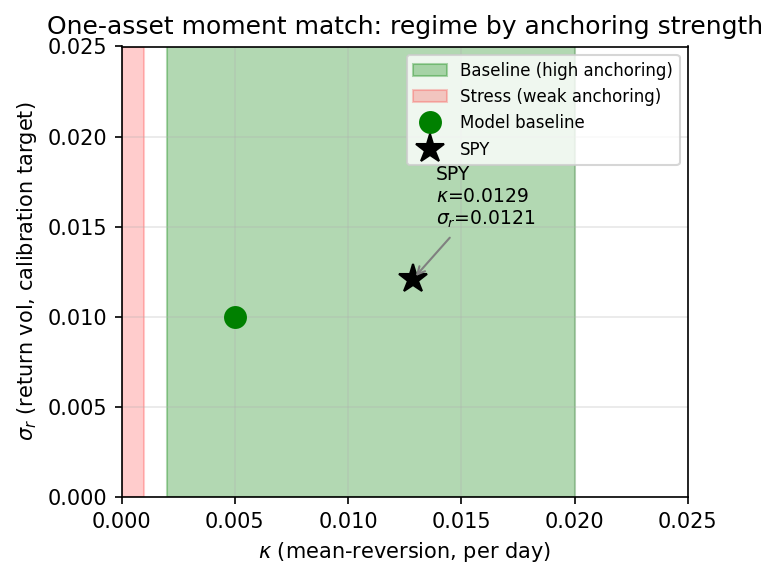
\includegraphics[width=0.48\textwidth]{../paper_artifacts/moment_match/fig_moment_match_regime.png}
  \caption{One-asset moment match: estimated $\kappa$ for SPY vs.\ baseline and stress regions (regime by anchoring strength). $\sigma_r$ shown as calibration target.}
  \label{fig:moment_match_regime}
\end{figure}


\subsection{Parameter regimes and stress diagnostics}
\label{sec:meaningful_regions}

\paragraph{Preview of findings.}
Two distinct notions matter in this model:
(i) \emph{level amplification}---large mispricing/volatility levels under weak anchoring and/or high noise trading; and
(ii) \emph{overconfidence (treatment) effects}---differences in outcomes when increasing perceived signal precision from $k=1$ to $k=3$.
Our simulations show substantial \emph{level amplification} under stress regimes (Table~\ref{tab:mispricing_stress}), while the incremental
$k$-effects on average mispricing are modest in both baseline and stress calibrations (Tables~\ref{tab:metrics}--\ref{tab:mispricing_persistence}).

\subsubsection{Stress regimes: when mispricing \emph{levels} become economically large}
\label{subsec:stress}
Table~\ref{tab:mispricing_stress} reports ``stress diagnostics'' in which anchoring is weakened ($\kappa$ reduced) and/or noise trading increases ($\phi$ increased).
Weak anchoring and high $\phi$ generate large mispricing and volatility \emph{levels} (e.g., $\E[|p-v|]$ exceeding $3$--$9$ in stress cases vs.\ $\approx 1.9$ in baseline).
\textbf{Importantly, these level shifts are primarily driven by $(\kappa,\phi)$: within each stress case, outcomes are nearly unchanged between $k=1$ and $k=3$.}
This demonstrates that level amplification comes from market microstructure parameters (anchoring strength, noise trading) rather than the overconfidence treatment.

\subsubsection{Baseline benchmark: \texorpdfstring{$k$}{k} primarily increases disagreement and trading intensity}
\label{subsec:baseline_benchmark}
We next report the baseline bull/bear scenarios under the benchmark calibration (Table~\ref{tab:params}).
In this parameterization, increasing overconfidence primarily increases cross-sectional disagreement and trading intensity
(e.g., $\Delta \E[\sigma_i(\hat v_i)] \approx +0.059$ and $\Delta \E[\sigma_i(x_i)] \approx +0.001$), while changes in mean absolute mispricing remain modest ($|\Delta \E[|p-v|]| \approx 0.004$).
Mispricing tail and persistence diagnostics (Table~\ref{tab:mispricing_persistence}) are essentially unchanged across $k$.
This baseline serves as a robustness check: it demonstrates that the model does not always amplify mispricing, and that overconfidence's primary channel is through belief dispersion and trading intensity rather than price levels.

\subsubsection{Targeted joint-move grid: \texorpdfstring{$k$}{k}-effects on mispricing are robustly small}
\label{subsec:joint_grid}
A natural concern is that one-at-a-time sweeps may miss interaction effects: overconfidence-induced amplification might require
\emph{simultaneous} changes in anchoring strength, price impact, and noise trading. To test this directly, we run a targeted
$3\times 3\times 3$ grid over $(\kappa,\lambda,\phi)$ in the bull regime using paired random seeds and compare
$k=3$ against $k=1$ within each cell.

Table~\ref{tab:joint_grid} reports cell-by-cell differences in key diagnostics, and
Figures~\ref{fig:joint_grid_mispricing}--\ref{fig:joint_grid_disagreement} visualize the resulting treatment effects.
We classify a cell as \emph{non-negligible} if (i) the 95\% confidence interval for $\Delta_k \E[|p-v|]$ excludes zero and
(ii) $|\Delta_k \E[|p-v|]|$ exceeds 5\% of the baseline $\E[|p-v|]$ in the same cell.

\textbf{Negative result (robust across the joint grid).}
Across the full joint grid, $k=3-1$ differences in $\E[|p-v|]$ are economically small: in Table~\ref{tab:joint_grid}, $\Delta_k\E[|p-v|]$ ranges from $0$ to about $-0.02$ and only $2$ out of $27$ cells meet our ``non-negligible'' flag threshold.
In several cells the 95\% confidence interval excludes zero, but the magnitude remains small relative to the baseline mispricing level (order $1$--$10$ depending on the regime),
including in cells where weak anchoring and high noise trading generate large \emph{levels} of mispricing.
By contrast, disagreement and trading-intensity proxies move systematically with $k$.
In this architecture, overconfidence primarily loads onto belief dispersion and trading intensity rather than price-level mispricing.
% Optional robustness: (i) Bear-regime repeat of the same grid; (ii) Report largest $|\Delta_k \E[|p-v|]|$ cell even if below 5\% threshold.

\begin{table}[t]
  \centering
  \scriptsize
  \setlength{\tabcolsep}{3pt}
  \resizebox{\columnwidth}{!}{\begin{tabular}{rrrcccccc}
\hline
$\phi$ & $\kappa$ & $\lambda$ & $\Delta\E[|p-v|]$ & $\Delta\E[\sigma_i(\hat v_i)]$ & $\Delta\E[|x_i|]$ & $\Delta\,\mathrm{std}(\sum_i x_i)$ & $\Delta\,\mathrm{std}(r)$ & Flag \\
\hline
0.25 & 0.001 & 0.10 & $-0.000\pm0.004$ & $0.059\pm0.000$ & $0.000\pm0.000$ & $0.038\pm0.055$ & $-0.000\pm0.000$ &  \\
0.25 & 0.001 & 0.20 & $-0.004\pm0.005$ & $0.059\pm0.000$ & $0.000\pm0.000$ & $0.049\pm0.084$ & $-0.000\pm0.000$ &  \\
0.25 & 0.001 & 0.50 & $-0.013\pm0.004$ & $0.059\pm0.000$ & $0.001\pm0.001$ & $0.150\pm0.125$ & $0.000\pm0.000$ &  \\
0.25 & 0.005 & 0.10 & $-0.006\pm0.005$ & $0.059\pm0.000$ & $0.001\pm0.001$ & $0.230\pm0.247$ & $-0.000\pm0.000$ &  \\
0.25 & 0.005 & 0.20 & $-0.012\pm0.004$ & $0.059\pm0.000$ & $0.002\pm0.001$ & $0.394\pm0.297$ & $0.000\pm0.000$ &  \\
0.25 & 0.005 & 0.50 & $-0.019\pm0.003$ & $0.059\pm0.000$ & $0.002\pm0.001$ & $0.507\pm0.173$ & $0.001\pm0.000$ & $\checkmark$ \\
0.25 & 0.020 & 0.10 & $-0.012\pm0.003$ & $0.059\pm0.000$ & $0.007\pm0.003$ & $1.209\pm0.650$ & $0.000\pm0.000$ &  \\
0.25 & 0.020 & 0.20 & $-0.017\pm0.003$ & $0.059\pm0.000$ & $0.007\pm0.002$ & $1.197\pm0.435$ & $0.000\pm0.000$ &  \\
0.25 & 0.020 & 0.50 & $-0.019\pm0.003$ & $0.059\pm0.000$ & $0.004\pm0.002$ & $0.739\pm0.373$ & $0.001\pm0.001$ & $\checkmark$ \\
0.50 & 0.001 & 0.10 & $-0.000\pm0.001$ & $0.059\pm0.000$ & $0.000\pm0.000$ & $0.005\pm0.009$ & $-0.000\pm0.000$ &  \\
0.50 & 0.001 & 0.20 & $-0.001\pm0.003$ & $0.059\pm0.000$ & $0.000\pm0.000$ & $0.006\pm0.027$ & $-0.000\pm0.000$ &  \\
0.50 & 0.001 & 0.50 & $-0.002\pm0.004$ & $0.059\pm0.000$ & $0.000\pm0.000$ & $0.002\pm0.016$ & $-0.000\pm0.000$ &  \\
0.50 & 0.005 & 0.10 & $-0.001\pm0.002$ & $0.059\pm0.000$ & $0.000\pm0.000$ & $0.016\pm0.051$ & $-0.000\pm0.000$ &  \\
0.50 & 0.005 & 0.20 & $-0.005\pm0.005$ & $0.059\pm0.000$ & $0.000\pm0.001$ & $0.042\pm0.116$ & $-0.000\pm0.000$ &  \\
0.50 & 0.005 & 0.50 & $-0.007\pm0.005$ & $0.059\pm0.000$ & $0.000\pm0.000$ & $0.027\pm0.064$ & $-0.000\pm0.000$ &  \\
0.50 & 0.020 & 0.10 & $-0.003\pm0.002$ & $0.059\pm0.000$ & $0.001\pm0.001$ & $0.132\pm0.181$ & $-0.000\pm0.000$ &  \\
0.50 & 0.020 & 0.20 & $-0.008\pm0.004$ & $0.059\pm0.000$ & $0.001\pm0.001$ & $0.295\pm0.320$ & $0.000\pm0.000$ &  \\
0.50 & 0.020 & 0.50 & $-0.009\pm0.004$ & $0.059\pm0.000$ & $0.001\pm0.001$ & $0.152\pm0.154$ & $0.000\pm0.000$ &  \\
1.50 & 0.001 & 0.10 & $-0.000\pm0.000$ & $0.059\pm0.000$ & $0.000\pm0.000$ & $0.000\pm0.001$ & $-0.000\pm0.000$ &  \\
1.50 & 0.001 & 0.20 & $-0.000\pm0.000$ & $0.059\pm0.000$ & $0.000\pm0.000$ & $0.000\pm0.001$ & $-0.000\pm0.000$ &  \\
1.50 & 0.001 & 0.50 & $-0.000\pm0.000$ & $0.059\pm0.000$ & $0.000\pm0.000$ & $0.000\pm0.001$ & $-0.000\pm0.000$ &  \\
1.50 & 0.005 & 0.10 & $-0.000\pm0.000$ & $0.059\pm0.000$ & $0.000\pm0.000$ & $0.000\pm0.004$ & $-0.000\pm0.000$ &  \\
1.50 & 0.005 & 0.20 & $-0.000\pm0.000$ & $0.059\pm0.000$ & $0.000\pm0.000$ & $0.000\pm0.004$ & $-0.000\pm0.000$ &  \\
1.50 & 0.005 & 0.50 & $-0.001\pm0.001$ & $0.059\pm0.000$ & $0.000\pm0.000$ & $-0.000\pm0.004$ & $-0.000\pm0.000$ &  \\
1.50 & 0.020 & 0.10 & $-0.000\pm0.000$ & $0.059\pm0.000$ & $0.000\pm0.000$ & $0.004\pm0.016$ & $-0.000\pm0.000$ &  \\
1.50 & 0.020 & 0.20 & $-0.001\pm0.001$ & $0.059\pm0.000$ & $0.000\pm0.000$ & $0.004\pm0.016$ & $-0.000\pm0.000$ &  \\
1.50 & 0.020 & 0.50 & $-0.001\pm0.001$ & $0.059\pm0.000$ & $0.000\pm0.000$ & $0.004\pm0.017$ & $-0.000\pm0.000$ &  \\
\hline
\end{tabular}
}
  \caption{Joint-grid treatment effects $\Delta_k$ across $(\kappa,\lambda,\phi)$ (Bull regime; $\Delta$ denotes $k=3$ minus $k=1$; mean $\pm$ 95\% CI across paired seeds; ``Flag'' per thresholds in text).}
  \label{tab:joint_grid}
\end{table}

\begin{figure}[t]
  \centering
  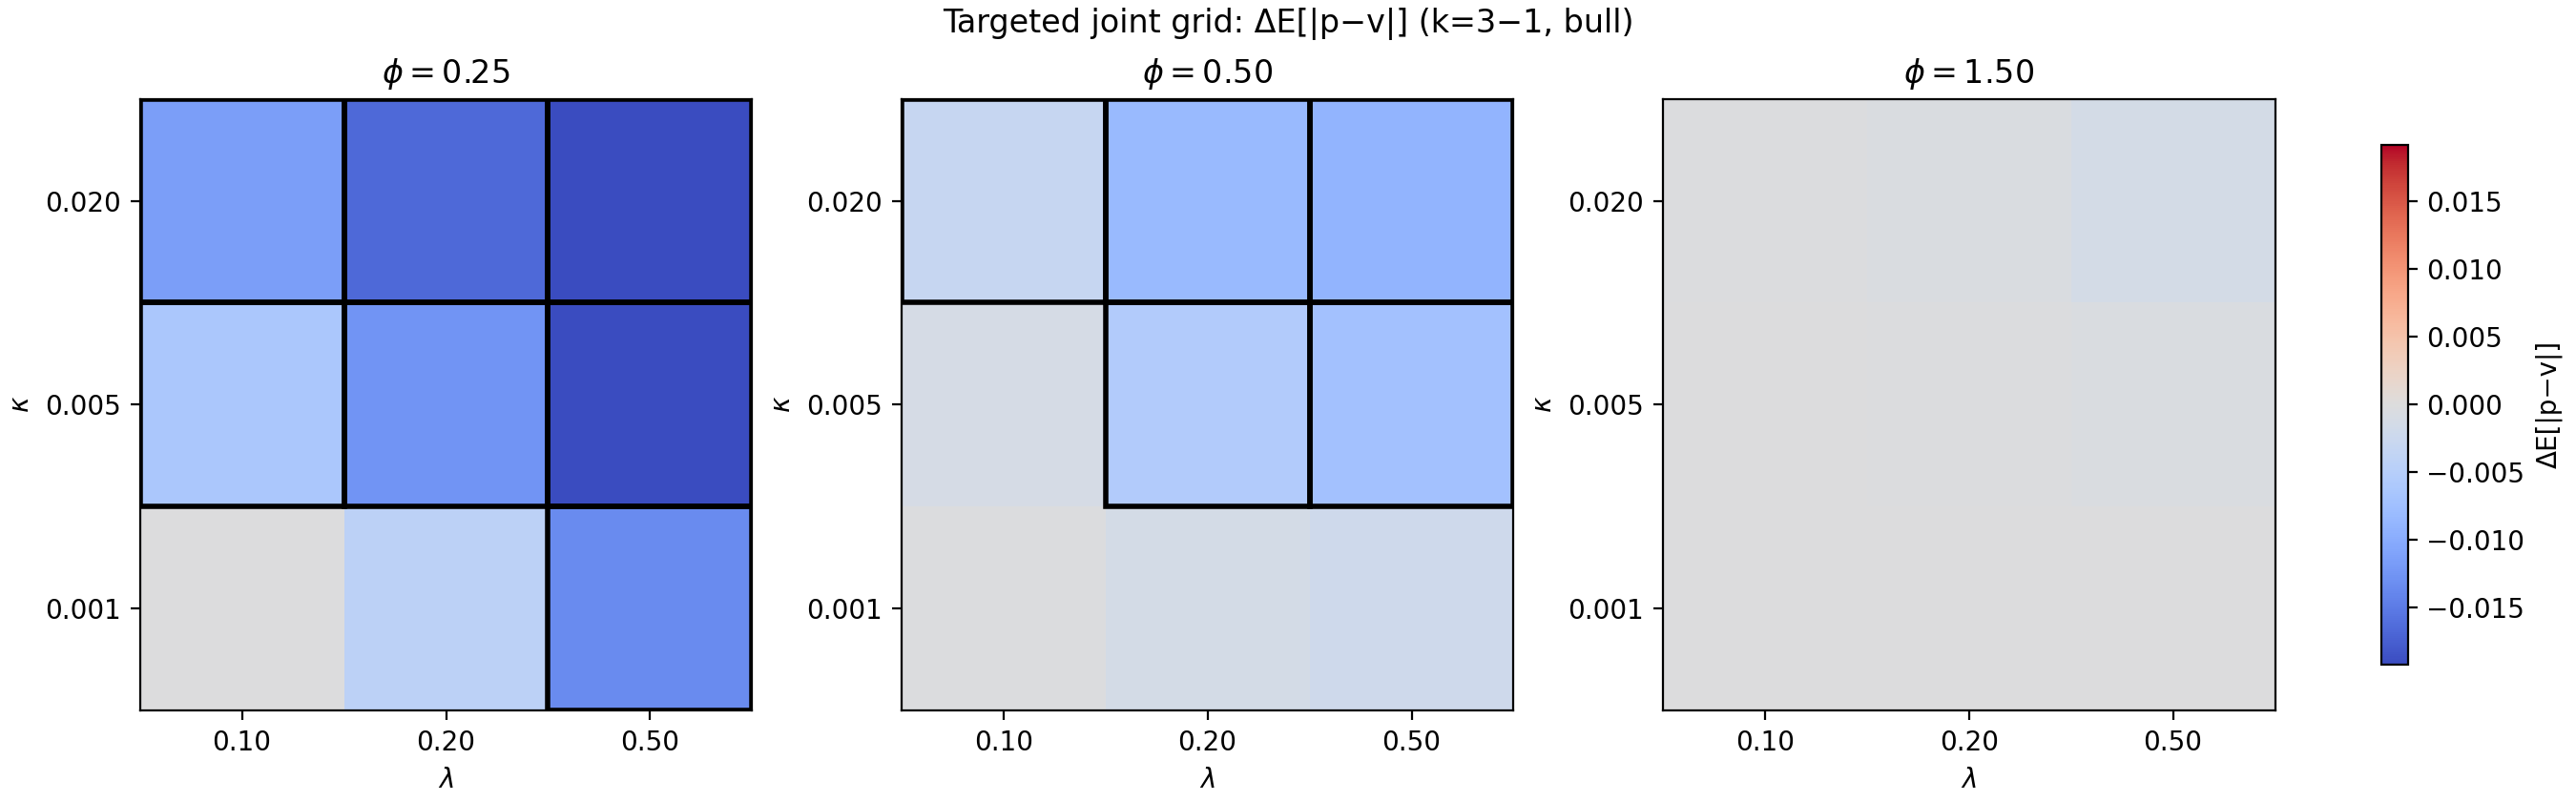
\includegraphics[width=0.95\linewidth]{../paper_artifacts/figures/fig_joint_move_grid_mispricing.png}
  \caption{Joint-grid treatment effects $\Delta_k \E[|p-v|]$ across $(\kappa,\lambda)$ for three $\phi$ slices.}
  \label{fig:joint_grid_mispricing}
\end{figure}

\begin{figure}[t]
  \centering
  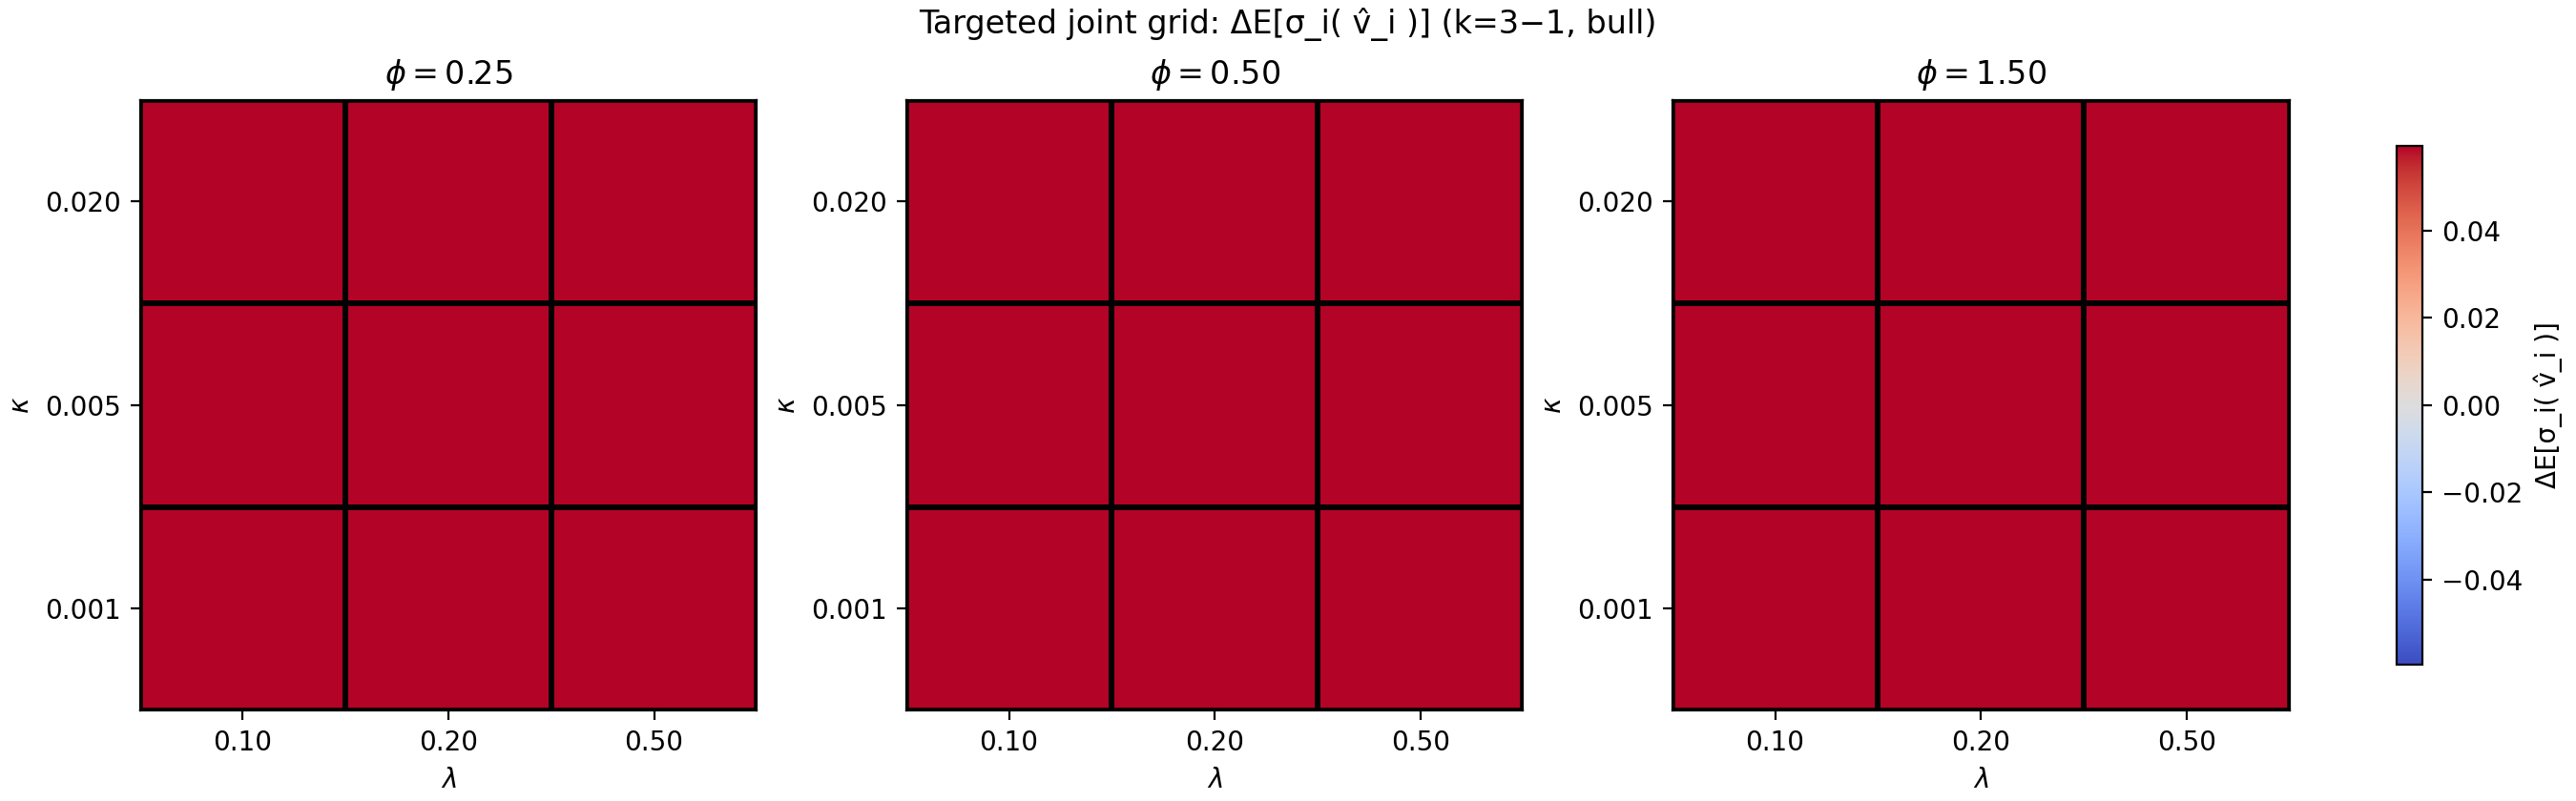
\includegraphics[width=0.95\linewidth]{../paper_artifacts/figures/fig_joint_move_grid_disagreement.png}
  \caption{Joint-grid treatment effects on disagreement $\Delta_k \E[\sigma_i(\hat v_i)]$ across $(\kappa,\lambda)$ for three $\phi$ slices.}
  \label{fig:joint_grid_disagreement}
\end{figure}

\subsubsection{One-at-a-time sweeps: why they rarely generate large \texorpdfstring{$k$}{k}-effects}
\label{subsec:sweeps}
The joint-grid above (Subsection~\ref{subsec:joint_grid}) establishes that we checked the obvious concern: simultaneous changes in $(\kappa,\lambda,\phi)$ do not reveal hidden $k$-driven mispricing amplification. We now report one-at-a-time sweeps over the key levers highlighted by the model: the impact-to-anchoring ratio $(\lambda/\kappa)$,
signal-to-noise in private information, anchoring strength $\kappa$, and regime drift magnitude $|\mu_v|$.

\textbf{Economic significance (Flag).}
The ``Flag'' column in Tables~\ref{tab:lambda_kappa_sweep}--\ref{tab:regime_strength_sweep} and in the joint grid (Table~\ref{tab:joint_grid}) marks cells where the $k=3{-}1$ effect is \emph{economically meaningful} by the following criteria.
\emph{Mispricing:} we flag if $|\Delta\E[|p-v|]| \ge \max(\theta_{\mathrm{abs}},\ \theta_{\mathrm{rel}}\times \text{baseline }\E[|p-v|])$.
For the one-at-a-time sweeps we use $\theta_{\mathrm{rel}}=10\%$ and $\theta_{\mathrm{abs}}=0.10$; for the joint grid we use $\theta_{\mathrm{rel}}=5\%$ and $\theta_{\mathrm{abs}}=0$ so that any cell with a nontrivial relative change in mispricing is flagged; the impaired-arbitrage extension (Table~\ref{tab:extension_state_dependent}) uses $\theta_{\mathrm{rel}}=5\%$ and $\theta_{\mathrm{abs}}=0.05$.
\emph{Return volatility:} we flag if $|\Delta\,\mathrm{std}(r)| \ge 20\%$ of the baseline $\mathrm{std}(r)$ in that cell.
These thresholds are chosen so that ``meaningful'' corresponds to a material relative change in mispricing (5--10\% of baseline) or a substantive change in return volatility (20\%); in our baseline, $\E[|p-v|]\approx 1.9$ (Table~\ref{tab:metrics}), so $\theta_{\mathrm{abs}}=0.10$ is about 5\% of baseline.
A sensitivity check using $\theta_{\mathrm{rel}}\in\{5\%,15\%\}$ for mispricing and 15\% or 25\% for return volatility leaves the set of flagged cells nearly unchanged in our sweeps; the conclusion that $k$-effects on mispricing are small is robust to these alternatives.

\textbf{Across one-at-a-time sweeps (Tables~\ref{tab:lambda_kappa_sweep}--\ref{tab:regime_strength_sweep}), $k$-effects on mispricing diagnostics remain small, consistent with the baseline's strong anchoring channel ($\kappa=0.005$) suppressing mispricing regardless of other parameters.}
Even when sweeping impact strength $\lambda$ up to $0.50$ (Table~\ref{tab:lambda_kappa_sweep}), the $k$-effect on mispricing remains small (often negative) because anchoring remains strong.
The sweeps therefore map where outcomes become fragile in \emph{levels} and clarify which parameters would need to be jointly re-estimated in a full calibration exercise targeting economically meaningful mispricing episodes.

\begin{table}[t]
  \centering
  \scriptsize
  \setlength{\tabcolsep}{3pt}
  \resizebox{\columnwidth}{!}{\begin{tabular}{rrcccccc}
\hline
$\lambda$ (impact) & $\lambda/\kappa$ & $\Delta\E[|p-v|]$ & $\Delta q_{0.95}(|p-v|)$ & $\Delta q_{0.99}(|p-v|)$ & $\Delta\,\mathrm{std}(r)$ & $\Delta\,\rho_1(|r|)$ & Flag \\
\hline
0.10 & 20.0 & $0.000\pm0.002$ & $-0.002\pm0.005$ & $-0.004\pm0.003$ & $-0.000\pm0.000$ & $-0.000\pm0.000$ &  \\
0.20 & 40.0 & $-0.000\pm0.005$ & $-0.012\pm0.012$ & $-0.009\pm0.015$ & $-0.000\pm0.000$ & $-0.000\pm0.000$ &  \\
0.30 & 60.0 & $0.000\pm0.005$ & $-0.002\pm0.012$ & $-0.008\pm0.010$ & $-0.000\pm0.000$ & $-0.000\pm0.000$ &  \\
0.40 & 80.0 & $-0.001\pm0.005$ & $-0.010\pm0.014$ & $-0.013\pm0.013$ & $-0.000\pm0.000$ & $-0.000\pm0.000$ &  \\
0.50 & 100.0 & $-0.001\pm0.006$ & $-0.009\pm0.012$ & $-0.013\pm0.018$ & $-0.000\pm0.000$ & $-0.000\pm0.000$ &  \\
0.75 & 150.0 & $-0.004\pm0.006$ & $-0.023\pm0.018$ & $-0.032\pm0.018$ & $-0.000\pm0.000$ & $0.000\pm0.001$ &  \\
1.00 & 200.0 & $-0.006\pm0.005$ & $-0.040\pm0.024$ & $-0.029\pm0.022$ & $0.000\pm0.000$ & $0.000\pm0.001$ &  \\
\hline
\end{tabular}
}
  \caption{Impact-to-anchoring sweep (Bull regime). $\Delta$ denotes $k=3$ minus $k=1$; ``Flag'' marks economically meaningful regions (see text for thresholds).}
  \label{tab:lambda_kappa_sweep}
\end{table}

\begin{figure}[t]
  \centering
  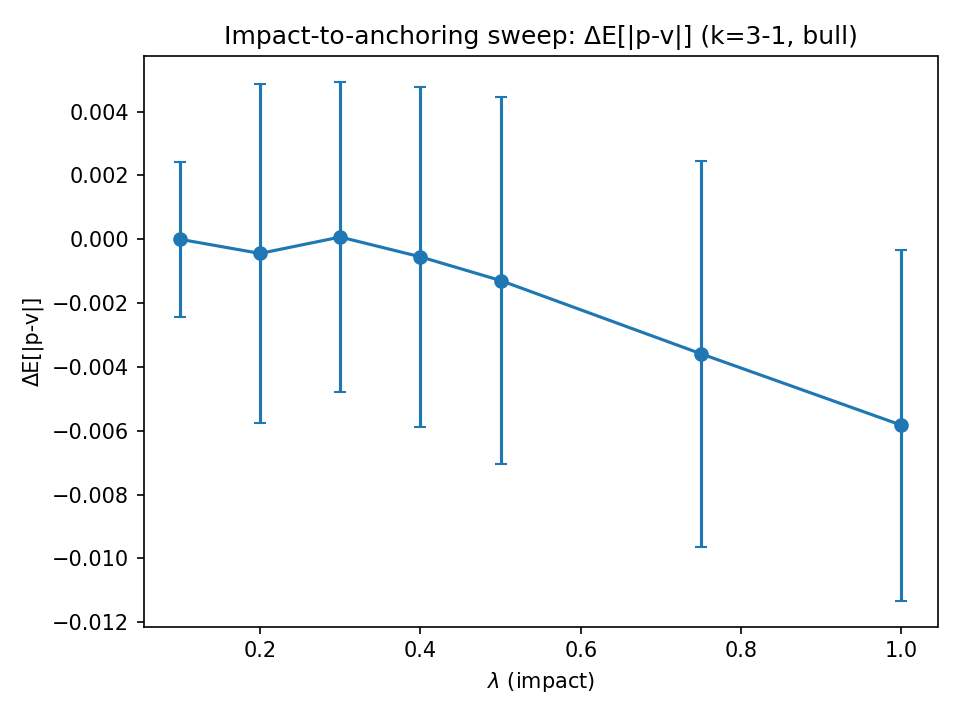
\includegraphics[width=0.48\textwidth]{../paper_artifacts/figures/fig_lambda_kappa_sweep_mispricing.png}
  \caption{Effect of $\lambda$ (impact) on $\Delta\E[|p-v|]$ (Bull regime; $\Delta$ denotes $k=3$ minus $k=1$).}
  \label{fig:lambda_kappa_sweep_mispricing}
\end{figure}

\begin{figure}[t]
  \centering
  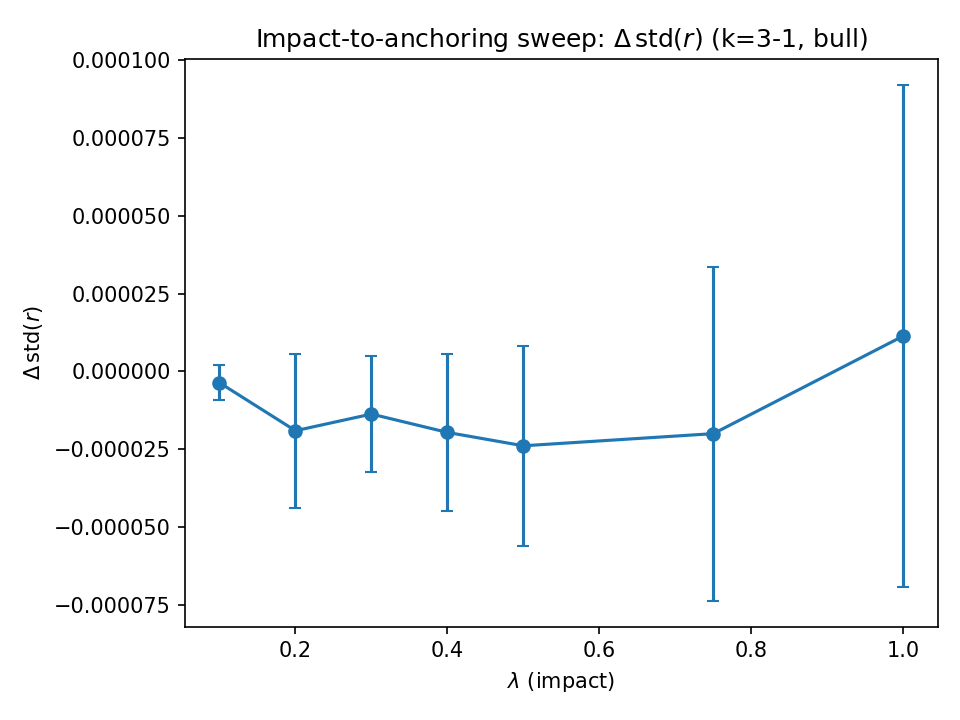
\includegraphics[width=0.48\textwidth]{../paper_artifacts/figures/fig_lambda_kappa_sweep_volatility.png}
  \caption{Effect of $\lambda$ (impact) on $\Delta\,\mathrm{std}(r)$ (Bull regime; $\Delta$ denotes $k=3$ minus $k=1$).}
  \label{fig:lambda_kappa_sweep_volatility}
\end{figure}

\begin{table}[t]
  \centering
  \scriptsize
  \setlength{\tabcolsep}{3pt}
  \resizebox{\columnwidth}{!}{\begin{tabular}{rrcccccccc}
\hline
$\sigma_\epsilon$ & $\sigma_v/\sigma_\epsilon$ & $\Delta\E[|p-v|]$ & $\Delta q_{0.95}(|p-v|)$ & $\Delta q_{0.99}(|p-v|)$ & $\Delta\,\mathrm{std}(r)$ & $\Delta\,\rho_1(|r|)$ & $\Delta\E[\sigma_i(\hat v_i)]$ & $\Delta\E[\sigma_i(x_i)]$ & Flag \\
\hline
0.40 & 0.250 & $-0.002\pm0.003$ & $-0.005\pm0.007$ & $-0.007\pm0.007$ & $-0.000\pm0.000$ & $-0.000\pm0.000$ & $0.037\pm0.000$ & $0.001\pm0.000$ &  \\
0.50 & 0.200 & $-0.003\pm0.003$ & $-0.008\pm0.009$ & $-0.007\pm0.007$ & $-0.000\pm0.000$ & $0.000\pm0.000$ & $0.044\pm0.000$ & $0.001\pm0.000$ &  \\
0.60 & 0.167 & $-0.003\pm0.004$ & $-0.009\pm0.011$ & $-0.007\pm0.009$ & $-0.000\pm0.000$ & $0.000\pm0.000$ & $0.050\pm0.000$ & $0.001\pm0.000$ &  \\
0.80 & 0.125 & $-0.004\pm0.006$ & $-0.009\pm0.013$ & $-0.007\pm0.012$ & $-0.000\pm0.000$ & $0.000\pm0.000$ & $0.060\pm0.000$ & $0.001\pm0.000$ &  \\
1.00 & 0.100 & $-0.005\pm0.007$ & $-0.009\pm0.013$ & $-0.009\pm0.014$ & $-0.000\pm0.000$ & $0.000\pm0.000$ & $0.068\pm0.000$ & $0.001\pm0.000$ &  \\
1.20 & 0.083 & $-0.005\pm0.008$ & $-0.007\pm0.015$ & $-0.010\pm0.016$ & $-0.000\pm0.000$ & $0.000\pm0.000$ & $0.075\pm0.000$ & $0.002\pm0.000$ &  \\
2.00 & 0.050 & $-0.007\pm0.012$ & $-0.021\pm0.022$ & $-0.021\pm0.017$ & $-0.000\pm0.000$ & $0.000\pm0.000$ & $0.100\pm0.000$ & $0.002\pm0.000$ &  \\
\hline
\end{tabular}
}
  \caption{Signal-to-noise sweep (Bull regime): varying $\sigma_\epsilon$ while holding $\sigma_v$ fixed. ``Flag'' marks economically meaningful regions (see text).}
  \label{tab:signal_to_noise_sweep}
\end{table}

\begin{figure}[t]
  \centering
  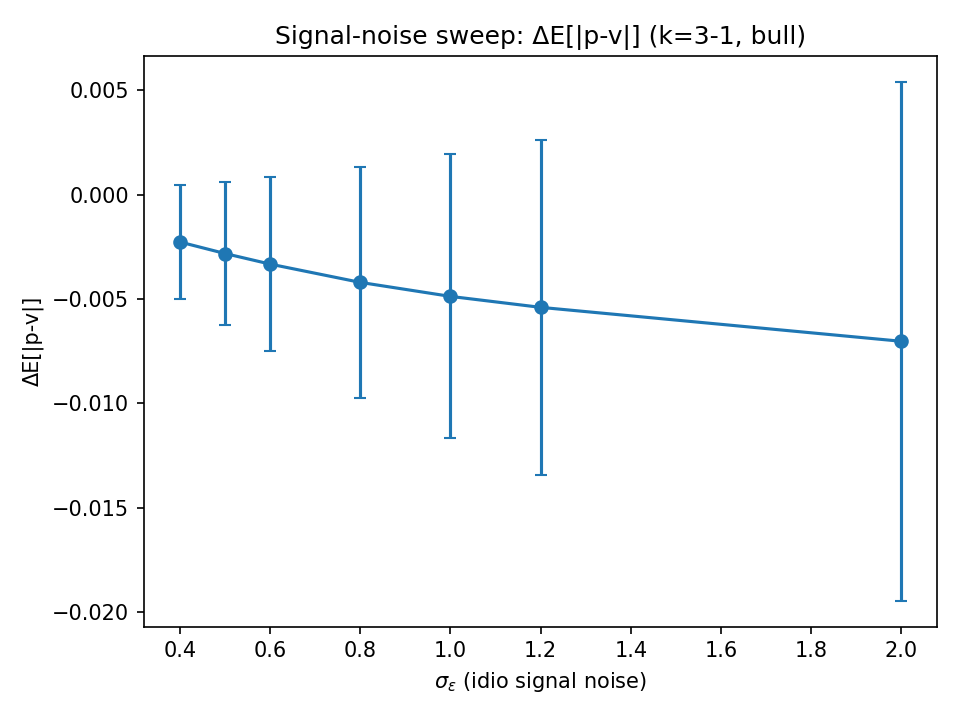
\includegraphics[width=0.48\textwidth]{../paper_artifacts/figures/fig_signal_to_noise_sweep_mispricing.png}
  \caption{Effect of $\sigma_\epsilon$ on $\Delta\E[|p-v|]$ (Bull regime; $\Delta$ denotes $k=3$ minus $k=1$).}
  \label{fig:signal_to_noise_sweep_mispricing}
\end{figure}

\begin{figure}[t]
  \centering
  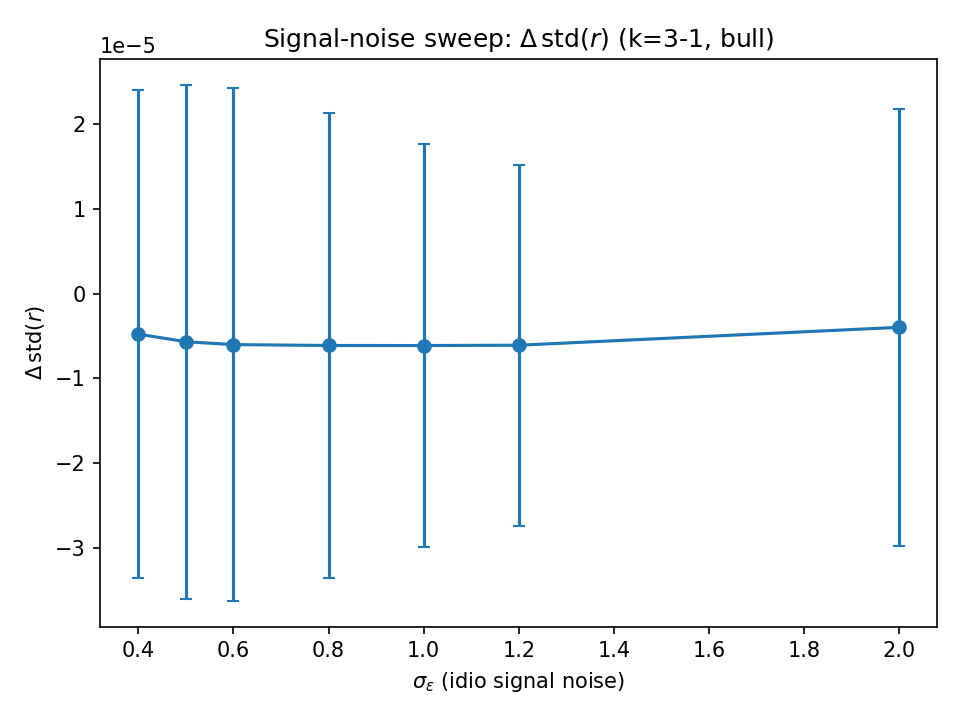
\includegraphics[width=0.48\textwidth]{../paper_artifacts/figures/fig_signal_to_noise_sweep_volatility.png}
  \caption{Effect of $\sigma_\epsilon$ on $\Delta\,\mathrm{std}(r)$ (Bull regime; $\Delta$ denotes $k=3$ minus $k=1$).}
  \label{fig:signal_to_noise_sweep_volatility}
\end{figure}

\begin{table}[t]
  \centering
  \scriptsize
  \setlength{\tabcolsep}{3pt}
  \resizebox{\columnwidth}{!}{\begin{tabular}{rrcccccc}
\hline
$\kappa$ & $\lambda/\kappa$ & $\Delta\E[|p-v|]$ & $\Delta q_{0.95}(|p-v|)$ & $\Delta q_{0.99}(|p-v|)$ & $\Delta\,\mathrm{std}(r)$ & $\Delta\,\rho_1(|r|)$ & Flag \\
\hline
0.001 & 200.0 & $0.001\pm0.003$ & $-0.003\pm0.005$ & $-0.002\pm0.006$ & $0.000\pm0.000$ & $0.000\pm0.000$ &  \\
0.002 & 100.0 & $0.000\pm0.004$ & $-0.000\pm0.007$ & $-0.004\pm0.007$ & $0.000\pm0.000$ & $0.000\pm0.000$ &  \\
0.003 & 66.7 & $-0.000\pm0.005$ & $-0.009\pm0.005$ & $-0.009\pm0.010$ & $0.000\pm0.000$ & $0.000\pm0.000$ &  \\
0.005 & 40.0 & $-0.002\pm0.004$ & $-0.010\pm0.011$ & $-0.015\pm0.010$ & $0.000\pm0.000$ & $0.000\pm0.000$ &  \\
0.010 & 20.0 & $-0.004\pm0.003$ & $-0.007\pm0.013$ & $-0.010\pm0.024$ & $0.000\pm0.000$ & $0.000\pm0.000$ &  \\
0.020 & 10.0 & $-0.004\pm0.003$ & $-0.011\pm0.014$ & $-0.017\pm0.025$ & $0.000\pm0.000$ & $-0.000\pm0.000$ &  \\
\hline
\end{tabular}
}
  \caption{Anchoring sweep (Bull regime): varying $\kappa$ at fixed $(\lambda,\phi)$. ``Flag'' marks economically meaningful regions (see text).}
  \label{tab:kappa_sweep}
\end{table}

\begin{table}[t]
  \centering
  \scriptsize
  \setlength{\tabcolsep}{3pt}
  \resizebox{\columnwidth}{!}{\begin{tabular}{lrcccccc}
\hline
Regime & $\mu_v$ & $\Delta\E[|p-v|]$ & $\Delta q_{0.95}(|p-v|)$ & $\Delta q_{0.99}(|p-v|)$ & $\Delta\,\mathrm{std}(r)$ & $\Delta\,\rho_1(|r|)$ & Flag \\
\hline
Bull & 0.010 & $-0.009\pm0.004$ & $-0.012\pm0.018$ & $-0.024\pm0.018$ & $-0.000\pm0.000$ & $-0.000\pm0.000$ &  \\
Bull & 0.020 & $-0.009\pm0.005$ & $-0.011\pm0.015$ & $-0.020\pm0.021$ & $-0.000\pm0.000$ & $-0.000\pm0.000$ &  \\
Bull & 0.030 & $-0.009\pm0.005$ & $-0.016\pm0.019$ & $-0.020\pm0.021$ & $-0.000\pm0.000$ & $-0.000\pm0.000$ &  \\
Bull & 0.050 & $-0.008\pm0.007$ & $-0.011\pm0.015$ & $-0.013\pm0.021$ & $-0.000\pm0.000$ & $-0.000\pm0.000$ &  \\
Bear & -0.010 & $-0.009\pm0.004$ & $-0.028\pm0.015$ & $-0.031\pm0.017$ & $-0.000\pm0.000$ & $-0.000\pm0.000$ &  \\
Bear & -0.020 & $-0.009\pm0.004$ & $-0.023\pm0.014$ & $-0.021\pm0.019$ & $-0.000\pm0.000$ & $-0.000\pm0.000$ &  \\
Bear & -0.030 & $-0.008\pm0.005$ & $-0.019\pm0.021$ & $-0.018\pm0.020$ & $-0.000\pm0.000$ & $-0.000\pm0.000$ &  \\
Bear & -0.050 & $-0.007\pm0.007$ & $-0.009\pm0.025$ & $-0.018\pm0.025$ & $-0.000\pm0.000$ & $-0.000\pm0.000$ &  \\
\hline
\end{tabular}
}
  \caption{Regime-strength sweep: varying $|\mu_v|$ in bull/bear regimes. ``Flag'' marks economically meaningful regions (see text).}
  \label{tab:regime_strength_sweep}
\end{table}

\begin{table}[t]
  \centering
  \scriptsize
  \setlength{\tabcolsep}{3pt}
  \resizebox{\columnwidth}{!}{\begin{tabular}{lrrcccccc}
\hline
Scenario & $\kappa$ & $\phi$ & \multicolumn{2}{c}{$\E[|p-v|]$} & \multicolumn{2}{c}{$q_{0.95}(|p-v|)$} & \multicolumn{2}{c}{$\mathrm{std}(r)$} \\
 &  &  & $k=1$ & $k=3$ & $k=1$ & $k=3$ & $k=1$ & $k=3$ \\
\hline
Baseline & 0.005 & 0.50 & $1.774\pm0.273$ & $1.767\pm0.276$ & $4.164\pm0.634$ & $4.155\pm0.633$ & $0.491\pm0.008$ & $0.491\pm0.008$ \\
Weak anchoring & 0.001 & 0.50 & $3.972\pm1.318$ & $3.969\pm1.320$ & $8.118\pm2.108$ & $8.113\pm2.112$ & $0.488\pm0.008$ & $0.488\pm0.008$ \\
High noise & 0.005 & 1.00 & $6.113\pm1.909$ & $6.112\pm1.910$ & $13.461\pm3.392$ & $13.460\pm3.393$ & $0.977\pm0.015$ & $0.977\pm0.015$ \\
Weak+high & 0.001 & 1.00 & $9.258\pm3.875$ & $9.258\pm3.875$ & $18.993\pm5.852$ & $18.993\pm5.851$ & $0.976\pm0.015$ & $0.976\pm0.015$ \\
Low noise & 0.005 & 0.25 & $0.614\pm0.049$ & $0.599\pm0.049$ & $1.514\pm0.145$ & $1.483\pm0.142$ & $0.249\pm0.004$ & $0.250\pm0.004$ \\
Mid-high noise & 0.005 & 0.75 & $4.377\pm1.290$ & $4.376\pm1.291$ & $9.706\pm2.366$ & $9.704\pm2.367$ & $0.733\pm0.012$ & $0.733\pm0.012$ \\
Very high noise & 0.005 & 1.50 & $9.308\pm2.886$ & $9.307\pm2.886$ & $20.516\pm5.137$ & $20.516\pm5.137$ & $1.465\pm0.023$ & $1.465\pm0.023$ \\
Extreme noise & 0.005 & 2.00 & $12.452\pm3.763$ & $12.452\pm3.763$ & $27.326\pm6.779$ & $27.326\pm6.779$ & $1.954\pm0.031$ & $1.954\pm0.031$ \\
Very weak anchoring & 0.001 & 0.50 & $4.999\pm1.827$ & $4.997\pm1.828$ & $9.910\pm2.868$ & $9.907\pm2.870$ & $0.488\pm0.008$ & $0.488\pm0.008$ \\
\hline
\end{tabular}
}
  \caption{Stress diagnostics: weakening anchoring ($\kappa$) and/or increasing noise trading ($\phi$) can generate large
mispricing and volatility \emph{levels}. Within each stress case, outcomes are nearly unchanged between $k=1$ and $k=3$,
indicating that level amplification is primarily driven by $(\kappa,\phi)$ rather than the overconfidence treatment.}
  \label{tab:mispricing_stress}
\end{table}

\begin{table}[t]
  \centering
  \scriptsize
  \setlength{\tabcolsep}{3pt}
  \resizebox{\columnwidth}{!}{\begin{tabular}{lccccc}
\hline
Case & $\E[|p-v|]$ & $q_{0.95}(|p-v|)$ & $q_{0.99}(|p-v|)$ & $\mathrm{std}(r)$ & $\mathrm{std}_{\mathrm{xs}}(k_i)$ \\
\hline
Fixed k=2.0 & $1.910\pm0.234$ & $4.475\pm0.546$ & $5.380\pm0.685$ & $0.504\pm0.011$ & $0.000\pm0.000$ \\
Uniform[1,3] (mean 2) & $1.658\pm0.183$ & $4.027\pm0.416$ & $5.007\pm0.549$ & $0.499\pm0.012$ & $0.563\pm0.009$ \\
Normal(2,0.5) clipped[1,3] & $1.658\pm0.183$ & $4.027\pm0.417$ & $5.007\pm0.549$ & $0.499\pm0.012$ & $0.469\pm0.015$ \\
\hline
\end{tabular}
}
  \caption{Heterogeneous $k$ at fixed mean $\E[k]=2$: comparing dispersion in confidence under the same market regime. Column $\mathrm{std}_{\mathrm{xs}}(k_i)$ is the cross-sectional standard deviation of $k_i$ across agents, time-averaged.}
  \label{tab:heterogeneous_k}
\end{table}

\subsection{Extensions and Validation Checks}
\label{subsec:extensions}

\subsubsection{Myopic vs.\ intertemporal policy}
The core qualitative decomposition is robust across equilibrium concepts: the main $k$-loading remains on disagreement and trading intensity; price-level mispricing is comparatively less sensitive to $k$ under both myopic and intertemporal LQG policies.
Comparisons use the same random seeds (paired shocks) and regime parameters; only the policy toggle and $k$ differ.
Table~\ref{tab:myopic_intertemporal} and Figures~\ref{fig:myopic_intertemporal_mispricing}--\ref{fig:myopic_intertemporal_decomposition} report the results.
The policy decomposition (Figure~\ref{fig:myopic_intertemporal_decomposition}) confirms the intertemporal hedging term is numerically active.
Mispricing is slightly lower under the intertemporal policy than under the myopic rule, and the $k$-treatment effect remains tiny under both; the modest negative $\Delta\E[|p-v|]$ when increasing $k$ is consistent with stronger perceived precision inducing faster corrective trading against mispricing under strong anchoring, so price levels do not blow out---what changes with $k$ is dispersion and trading intensity rather than the level of mispricing.

\begin{table}[t]
  \centering
  \scriptsize
  \setlength{\tabcolsep}{3pt}
  \resizebox{\columnwidth}{!}{\begin{tabular}{lcccc}
\hline
Policy & $k$ & $\mathbb{E}[|p-v|]$ & $q_{0.95}(|p-v|)$ & $\mathrm{std}(r)$ \\
\hline
Myopic & $1$ & $1.633\pm0.246$ & $3.622\pm0.583$ & $0.493\pm0.015$ \\
Myopic & $3$ & $1.632\pm0.246$ & $3.624\pm0.579$ & $0.493\pm0.016$ \\
Intertemporal & $1$ & $1.284\pm0.132$ & $2.868\pm0.313$ & $0.496\pm0.016$ \\
Intertemporal & $3$ & $1.290\pm0.134$ & $2.878\pm0.311$ & $0.496\pm0.016$ \\
$\Delta$ Myopic ($k=3-1$) & --- & $-0.001\pm0.002$ & $0.002\pm0.011$ & $0.000\pm0.000$ \\
$\Delta$ Intertemporal ($k=3-1$) & --- & $0.006\pm0.004$ & $0.010\pm0.012$ & $-0.000\pm0.000$ \\
\hline
\end{tabular}
}
  \caption{Myopic vs.\ intertemporal policy: $\E[|p-v|]$, $q_{0.95}(|p-v|)$, and $\mathrm{std}(r)$ by policy and $k$.}
  \label{tab:myopic_intertemporal}
\end{table}

\begin{figure}[t]
  \centering
  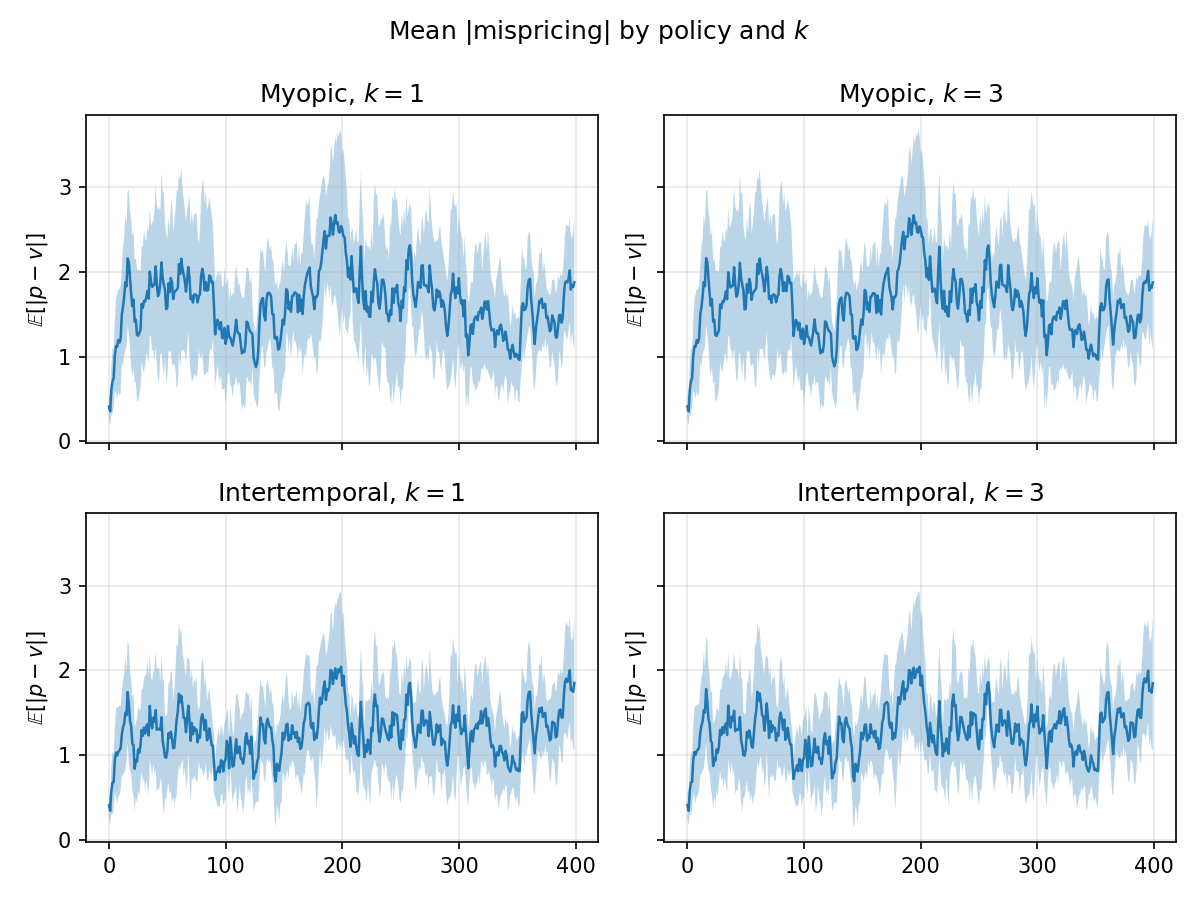
\includegraphics[width=0.95\linewidth]{../paper_artifacts/figures/fig_myopic_intertemporal_mispricing.png}
  \caption{Mean $|p-v|$ by policy (myopic/intertemporal) and $k$ (2$\times$2 grid; 95\% CI bands).}
  \label{fig:myopic_intertemporal_mispricing}
\end{figure}

\begin{figure}[t]
  \centering
  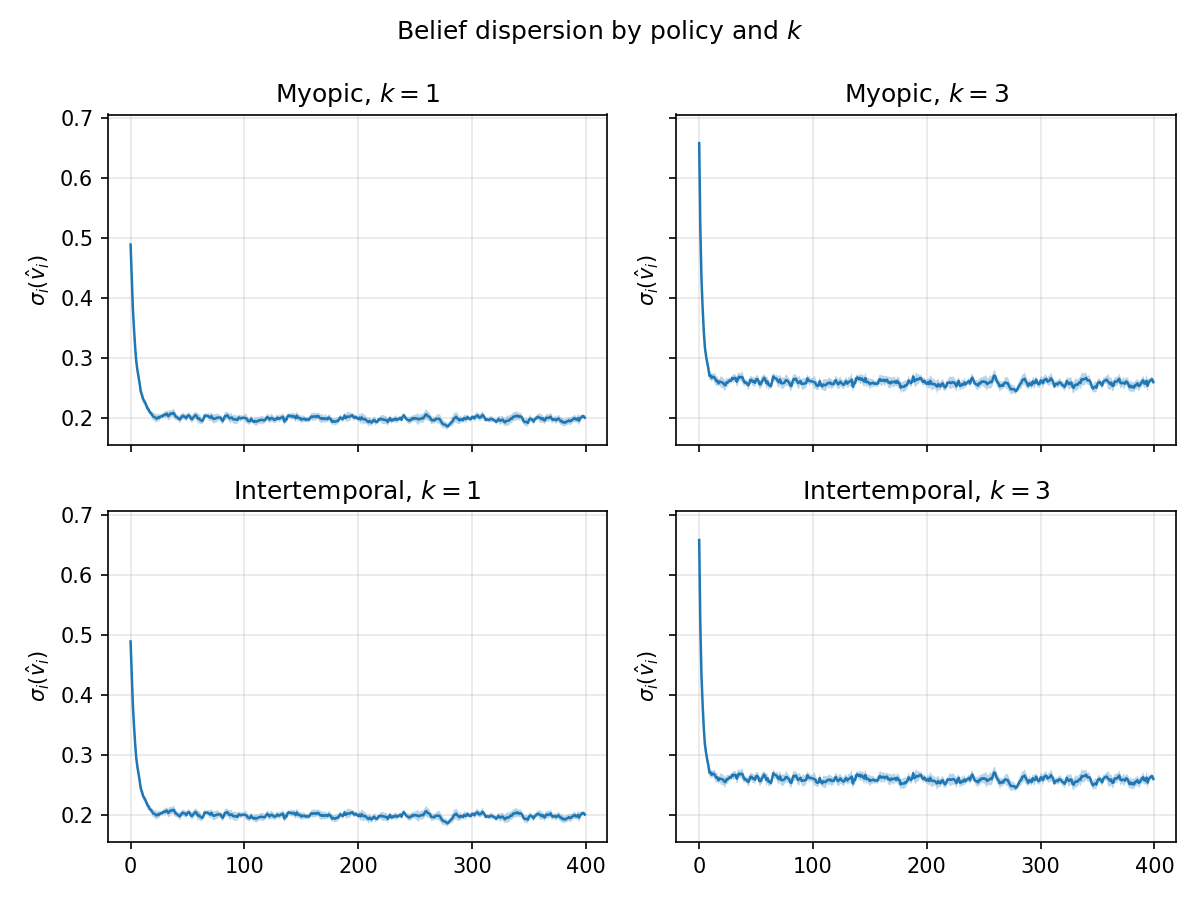
\includegraphics[width=0.95\linewidth]{../paper_artifacts/figures/fig_myopic_intertemporal_disagreement.png}
  \caption{Belief dispersion $\sigma_i(\hat v_i)$ by policy and $k$.}
  \label{fig:myopic_intertemporal_disagreement}
\end{figure}

\begin{figure}[t]
  \centering
  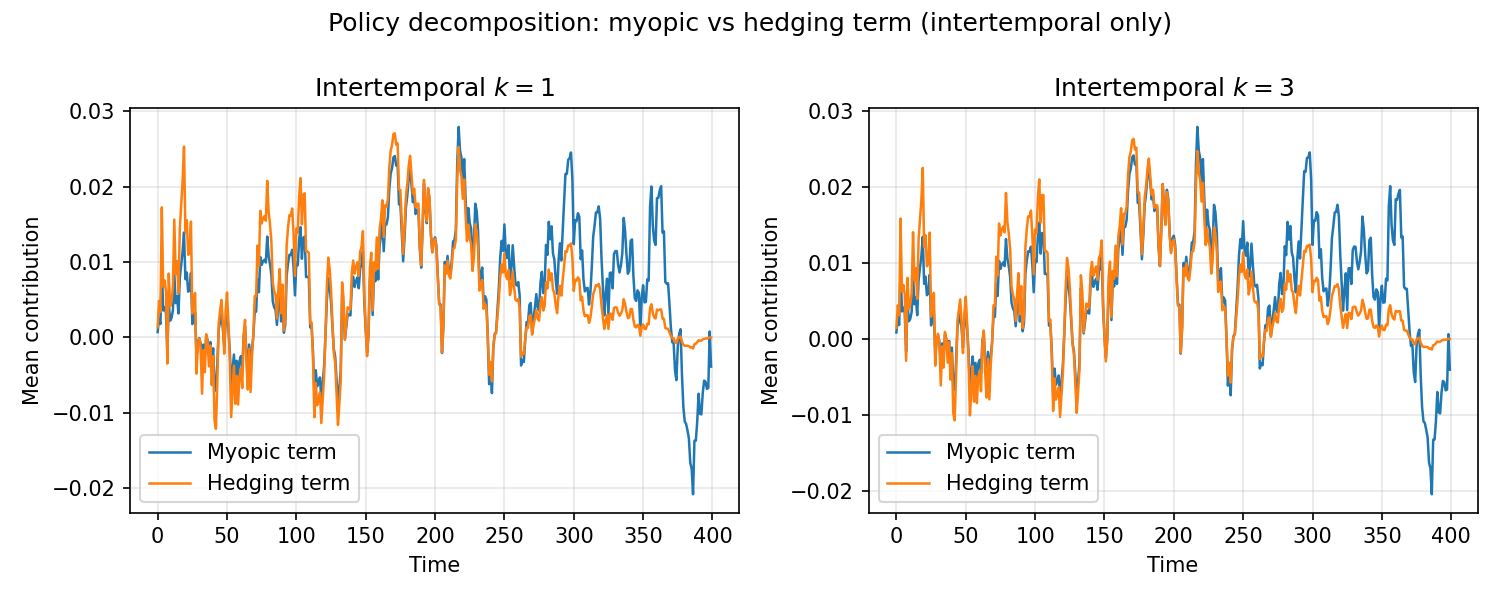
\includegraphics[width=0.95\linewidth]{../paper_artifacts/figures/fig_myopic_intertemporal_policy_decomposition.png}
  \caption{Policy decomposition: myopic vs.\ hedging term contribution (intertemporal runs).}
  \label{fig:myopic_intertemporal_decomposition}
\end{figure}

\subsubsection{Extension: when \texorpdfstring{$k$}{k} can move mispricing}
In the baseline anchored-impact microstructure (relevant for SPY-like regimes), $k$ does not materially move mispricing.
When arbitrage pressure is impaired---e.g., via state-dependent anchoring $\kappa(t)=\kappa_0\exp(-\alpha|p-v|)$ so that $\kappa$ weakens under large mispricing---$k$ can in principle transmit into price-level mispricing.
Table~\ref{tab:extension_state_dependent} and Figure~\ref{fig:extension_state_dependent} report the sensitivity to $\alpha$.
In the parameter range shown ($\alpha\in[0,0.2]$), $\Delta\E[|p-v|]$ ($k=3{-}1$) remains small (around $-0.004$ to $-0.005$); even under modest state-dependence, $k$-effects on mispricing stay small. Larger arbitrage impairment (e.g., higher $\alpha$, lower baseline $\kappa_0$, or higher $\phi$) would be required for $k$ to materially amplify mispricing. The negative result is not built into linearity; it is regime-specific: in the baseline (strong anchoring), $k$ loads onto disagreement/intensity; in sufficiently impaired-arbitrage regimes, $k$ can amplify mispricing.

\begin{table}[t]
  \centering
  \scriptsize
  \setlength{\tabcolsep}{3pt}
  \resizebox{\columnwidth}{!}{\begin{tabular}{rcccccc}
\hline
$\alpha$ & $\E[|p-v|]$ ($k=1$) & $\Delta\E[|p-v|]$ & $\Delta q_{0.5}$ & $\Delta q_{0.95}$ & Flag \\
\hline
0.00 & $1.655$ & $-0.003\pm0.005$ & $-0.000$ & $-0.011$ & $\checkmark$ \\
0.05 & $1.682$ & $-0.003\pm0.005$ & $-0.002$ & $-0.013$ & $\checkmark$ \\
0.10 & $1.707$ & $-0.003\pm0.005$ & $-0.003$ & $-0.010$ & $\checkmark$ \\
0.20 & $1.746$ & $-0.004\pm0.005$ & $0.006$ & $-0.010$ & $\checkmark$ \\
\hline
\end{tabular}
}
  \caption{Impaired-arbitrage extension: $\Delta\E[|p-v|]$ ($k=3{-}1$) vs.\ $\alpha$ (kappa decay rate). ``Flag'' per thresholds in text.}
  \label{tab:extension_state_dependent}
\end{table}

\begin{figure}[t]
  \centering
  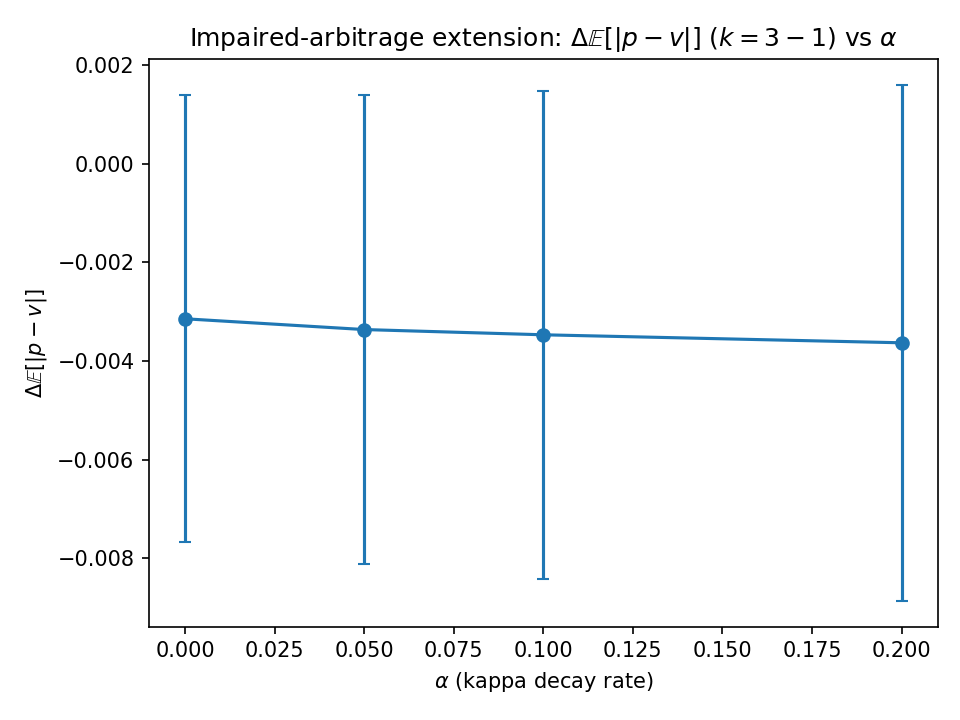
\includegraphics[width=0.48\textwidth]{../paper_artifacts/figures/fig_extension_state_dependent.png}
  \caption{Impaired-arbitrage extension: $\Delta\E[|p-v|]$ ($k=3-1$) vs.\ $\alpha$.}
  \label{fig:extension_state_dependent}
\end{figure}

\subsubsection{Empirical stylized fact: volume and realized return volatility co-movement}
We document a stylized fact consistent with the model's disagreement/intensity channel: volume (log volume) and realized return volatility (rolling standard deviation of daily log returns) co-move positively.
We cannot directly measure belief dispersion without survey/analyst microdata; we use uncertainty proxies as a reduced-form correlate.
This is a well-known generic relationship; we pitch it as external-face validity / sanity check for the model's intensity channel, not as an identification of ``disagreement.'' Analyst forecast dispersion, options-implied disagreement, or survey-based disagreement are natural next steps for tighter empirical tests.
Stress episodes are defined mechanically as the top decile of realized return volatility (no cherry-picking).

\begin{figure}[t]
  \centering
  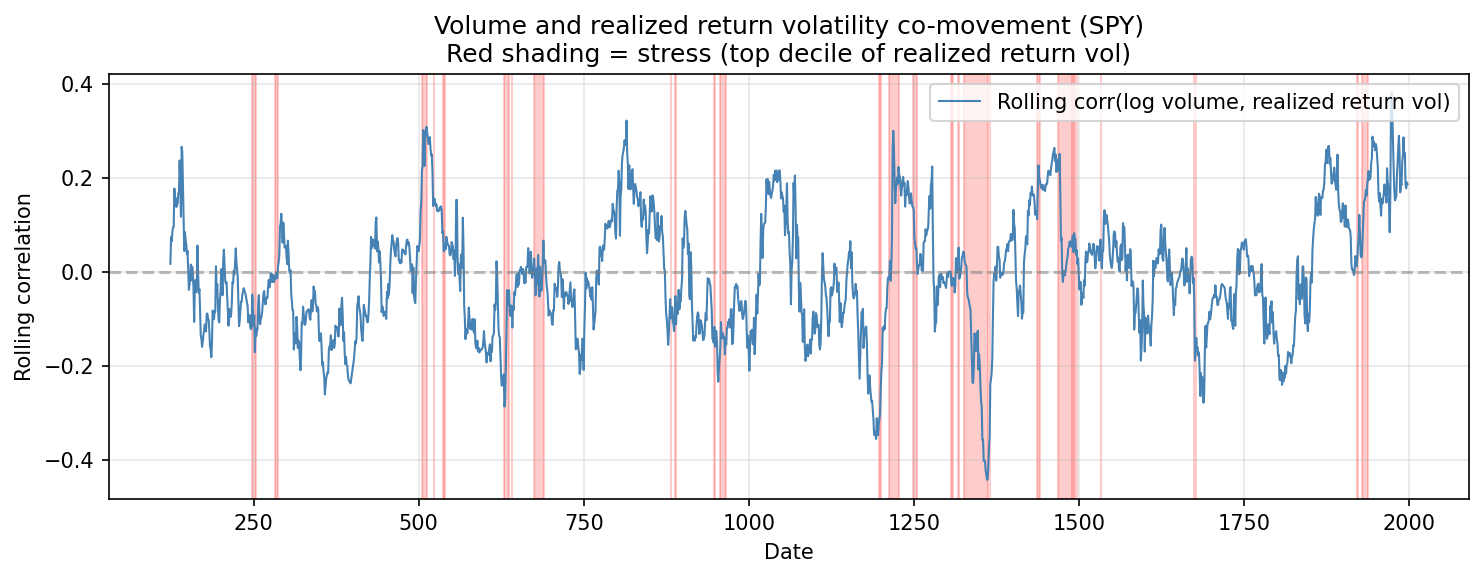
\includegraphics[width=0.95\linewidth]{../paper_artifacts/figures/fig_stylized_volume_volatility.png}
  \caption{Rolling correlation of log volume and realized return volatility (SPY). Red shading = stress (top decile of realized return vol).}
  \label{fig:stylized_volume_volatility}
\end{figure}

\begin{table}[t]
  \centering
  \scriptsize
  \setlength{\tabcolsep}{3pt}
  \resizebox{\columnwidth}{!}{\begin{tabular}{lccc}
\hline
Sample & Correlation & SE & $t$-stat \\
\hline
Full & $-0.018$ & $0.023$ & $-0.766$ \\
Stress (top decile realized vol) & $-0.053$ & $0.073$ & $-0.727$ \\
Non-stress & $-0.025$ & $0.024$ & $-1.009$ \\
\hline
\end{tabular}
}
  \caption{Volume--volatility correlation (log volume vs realized return volatility): full sample, stress, and non-stress (Newey--West $t$-stats).}
  \label{tab:stylized_volume_volatility}
\end{table}

Figure~\ref{fig:stylized_volume_volatility} plots the rolling correlation; Table~\ref{tab:stylized_volume_volatility} reports correlations in stress vs.\ non-stress with Newey--West $t$-statistics.
Our model provides a mechanism: overconfidence increases disagreement and trading intensity; when both are high, volume and belief dispersion move together.

\textbf{Baseline results (benchmark).} Figure~\ref{fig:price_path} reports the mean price path across baseline scenarios. Figure~\ref{fig:mispricing} reports mean absolute mispricing $\E[|p_t-v_t|]$ (computed from the simulated fundamental), and Figure~\ref{fig:volatility} reports a rolling volatility proxy based on realized returns.
Table~\ref{tab:metrics} complements the plots with seed-averaged moments and treatment effects ($k=3$ vs.\ $k=1$). 
\textbf{In this baseline parameterization, the $k$-effect on mispricing is weak ($|\Delta \E[|p-v|]| \approx 0.004$), and mispricing tail/persistence diagnostics (Table~\ref{tab:mispricing_persistence}) are essentially unchanged across $k$.}
Proposition~\ref{prop:mechanism_k} explains this analytically: the mean-field closure depends only on the mean belief $m_t-p_t$, so mispricing is driven by microstructure $(\kappa,\lambda,\phi)$ and the mean-belief error $e_t=m_t-v_t$; under the filter structure, $k$ raises disagreement (strictly in $k$) and trading intensity while affecting the mean belief only weakly, hence small price effects.
Increasing overconfidence primarily increases cross-sectional disagreement and trading intensity (e.g., $\Delta \E[\sigma_i(\hat v_i)] \approx +0.059$ and lower perceived $\E[\bar\Sigma]$), consistent with that mechanism.
The qualitative asymmetry remains visible in paths: bull regimes exhibit more persistent overvaluation episodes, while bear regimes exhibit noisier oscillations around fundamentals.

\begin{figure}[t]
  \centering
  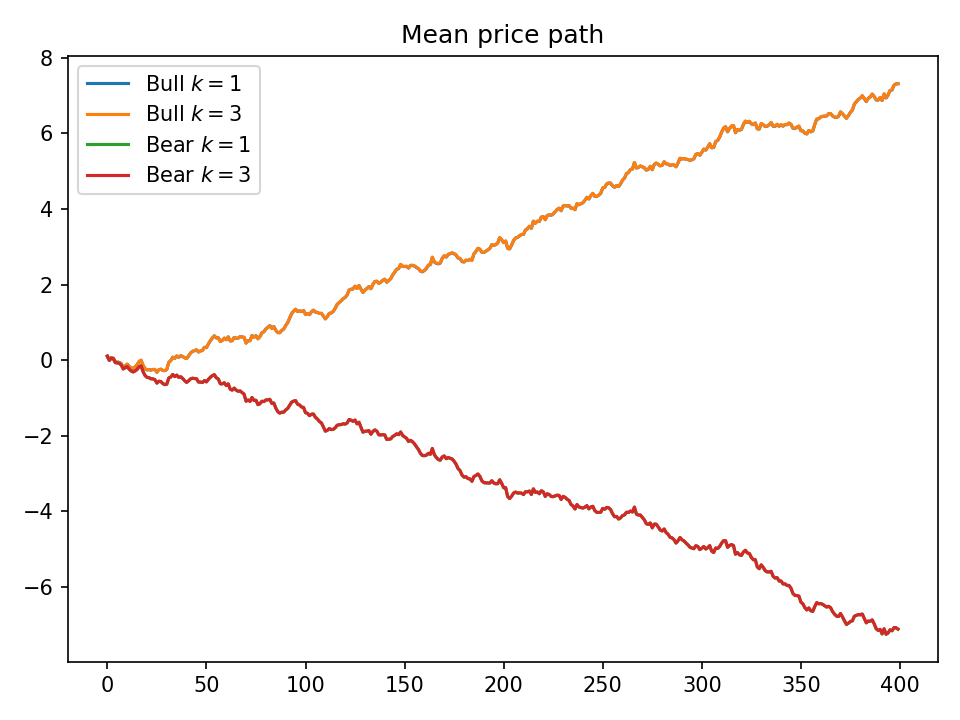
\includegraphics[width=0.48\textwidth]{../paper_artifacts/figures/fig_price_path.png}
  \caption{Mean price path across baseline scenarios (bull/bear regimes; $k\in\{1,3\}$).}
  \label{fig:price_path}
\end{figure}

\begin{figure}[t]
  \centering
  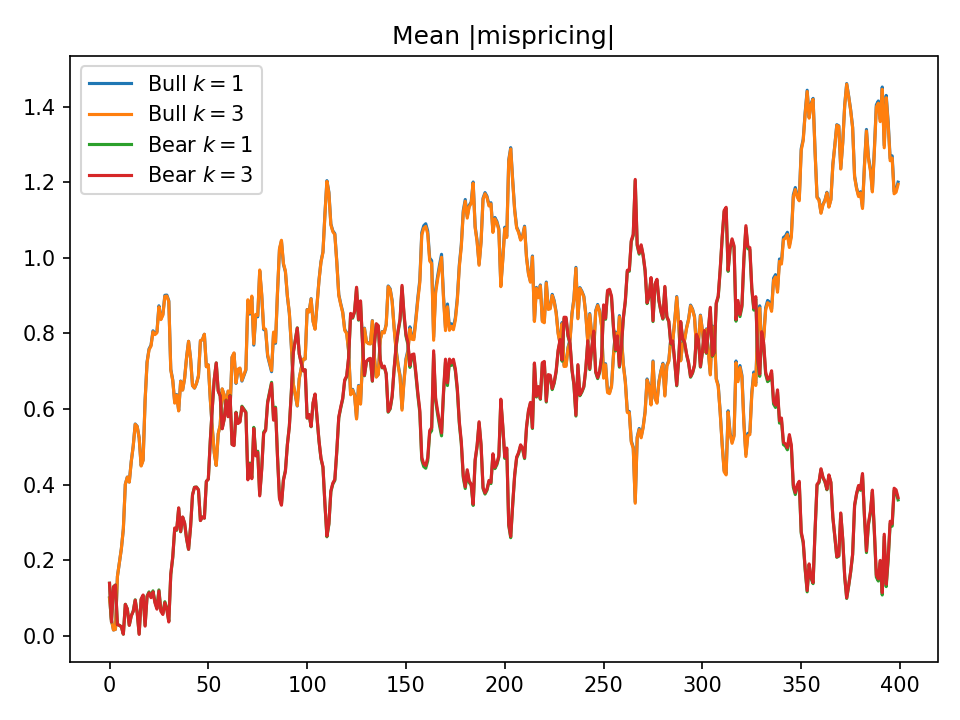
\includegraphics[width=0.48\textwidth]{../paper_artifacts/figures/fig_mispricing.png}
  \caption{Mean absolute mispricing $\E[|p_t-v_t|]$ across baseline scenarios.}
  \label{fig:mispricing}
\end{figure}

\begin{figure}[t]
  \centering
  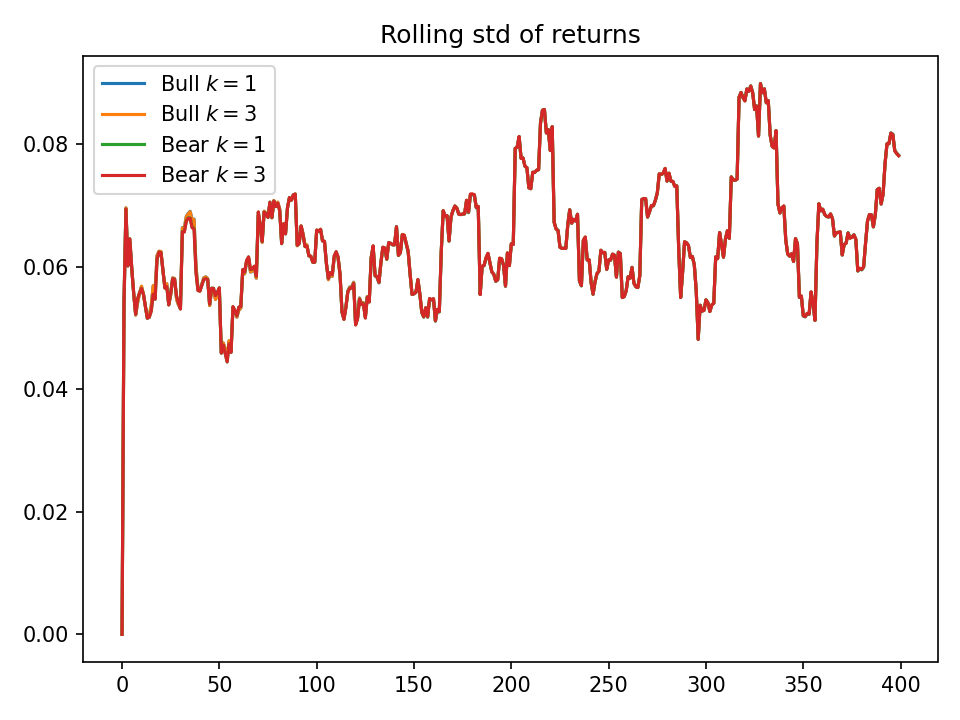
\includegraphics[width=0.48\textwidth]{../paper_artifacts/figures/fig_volatility.png}
  \caption{Rolling volatility proxy (standard deviation of returns) across baseline scenarios.}
  \label{fig:volatility}
\end{figure}

\textbf{Discussion.} The particle simulations are intended as computational evidence for the feedback mechanism highlighted by the model: misperceived signal precision affects belief dispersion and demand, which in turn impacts prices through \eqref{eq:anchored_impact}. A full numerical fixed-point verification for the common-noise mean-field limit (e.g., via conditional-law SPDE solvers) is left for future work.
As a robustness check for the informational simplification (filtering on $\xi_i$ only), the artifact script also produces a ``price-augmented'' filtering variant aligned with the Euler price update: it uses the realized increment $p_{t+1}-p_t$ to form an implicit noisy observation of $v_t$ (Appendix~A). The qualitative $k$-effects on perceived uncertainty and disagreement remain similar in that check (Table~\ref{tab:price_filter}).
